\documentclass[10pt,xcolor=svgnames]{beamer}
\usefonttheme{professionalfonts}
\usepackage[utf8]{inputenc}
\usepackage[T1]{fontenc}
\usepackage[french,english]{babel}
\usepackage{graphicx}
\usepackage{caption,subcaption}
\usepackage{animate}
\captionsetup{compatibility=false}

\usepackage[style=alphabetic,maxbibnames=99,backref=true,backend=biber]{biblatex}
\AtBeginBibliography{\footnotesize}
\addbibresource{main.bib}

\usepackage[linesnumbered,commentsnumbered,ruled,vlined]{algorithm2e}
\usepackage[linewidth=2.5pt,linecolor=black,nobreak=true]{mdframed}
\mdfsetup{frametitlealignment=\center}

\usepackage{amstext,amsmath,amssymb,bm,bbm,graphicx,mathtools,accents}
\usepackage{beamerleanprogress}
\usepackage{tikz}
\usepackage{transparent}

%%%%%%%  Environments  %%%%%%%%%%%

\newcounter{definition}[section]
\newenvironment{definition}[1]{\refstepcounter{definition} \par\bigskip \noindent  \begin{minipage}[b]{\linewidth} 
\textbf{Definition~\thedefinition(#1):}}{\end{minipage} \par\bigskip}

\newcounter{example}[section]
\newenvironment{example}{\refstepcounter{example} \par\medskip
\noindent  \begin{minipage}[b]{\linewidth} \textbf{Example~\theexample :}}{\end{minipage} \par\bigskip}

\newcounter{proposition}[section]
\newenvironment{proposition}[1]{\refstepcounter{proposition} \par\medskip \noindent  \begin{minipage}[b]{\linewidth} \textbf{Proposition~\theproposition(#1):}}{\end{minipage} \par\bigskip}

\newcounter{theorem}[section]
\newenvironment{theorem}[1]{\refstepcounter{theorem} \par\medskip \noindent  \begin{minipage}[b]{\linewidth} \textbf{Theorem~\thetheorem(#1):}}{\end{minipage} \par\bigskip}

\newenvironment{proof}{\noindent\ignorespaces\textit{Proof: }}{\hfill $\blacksquare$ \par\noindent\ignorespacesafterend\medskip}

\newcounter{assumption}[section]
\newenvironment{assumption}{ \refstepcounter{assumption} \renewcommand{\theequation}{A.\arabic{assumption}}}{\renewcommand{\theequation}{\arabic{section}.\arabic{equation}} }



%%%%%%%%%%%%%% Commands %%%%%%%%%%%
\newcommand{\daniel}[1]{{\color{black}{#1}}}
\newcommand{\revision}[1]{{\color{blue}{#1}}}

\newcommand{\transp}{\mathbf{T}}
\newcommand{\edge}[2]{ ( #1,#2 )}

\newcommand{\sketch}[1]{{\color{red}{#1}}}
\newcommand{\ol}[1]{{\overline{#1}}}
\newcommand{\av}[1]{\accentset{\circ}{\vec{#1}}}
\newcommand{\Ds}{D}
\newcommand\figTable[2]{\raisebox{-.5\height}{\includegraphics[scale=#1]{#2}}}


\DeclareMathOperator*{\argmin}{arg\,min}
\DeclareMathOperator*{\argmax}{arg\,max}
\renewcommand{\vec}[1]{\bm{#1}}
\DeclarePairedDelimiter\norm{\lVert}{\rVert}%
\DeclarePairedDelimiter\bignorm{\Big\lVert}{\Big\rVert}%
\DeclarePairedDelimiter\abs{\lvert}{\rvert}%

\newcommand{\GG}{ \mathcal{G}_{\vec{I}} }
\newcommand{\GGe}{ \mathcal{G}_{\vec{I}+} }
\newcommand{\GGc}[1]{ \mathcal{G}_C^{(#1)} }
\newcommand{\GGcc}{ \mathcal{G}_C}

\makeatletter
\DeclareFontFamily{U}{tipa}{}
\DeclareFontShape{U}{tipa}{m}{n}{<->tipa10}{}
\newcommand{\arc@char}{{\usefont{U}{tipa}{m}{n}\symbol{62}}}%

\newcommand{\arc}[1]{\mathpalette\arc@arc{#1}}

\newcommand{\arc@arc}[2]{%
  \sbox0{$\m@th#1#2$}%
  \vbox{
    \hbox{\resizebox{\wd0}{\height}{\arc@char}}
    \nointerlineskip
    \box0
  }%
}
\makeatother


%%%%%%%%%%% Misc %%%%%%%%%%%
\crefname{algocf}{alg.}{algs.}
\Crefname{algocf}{Algorithm}{Algorithms}
\Crefname{appsec}{Appendix}{Appendices}  

\setbeamertemplate{bibliography entry title}{}
\setbeamertemplate{bibliography entry location}{}
\setbeamertemplate{bibliography entry note}{}

\tikzset{
  invisible/.style={opacity=0},
  visible on/.style={alt={#1{}{invisible}}},
  alt/.code args={<#1>#2#3}{%
    \alt<#1>{\pgfkeysalso{#2}}{\pgfkeysalso{#3}} % \pgfkeysalso doesn't change the path
  },
}

\title
  [Geometric Constraints and Variational Approaches to Image Analysis]
  {Geometric Constraints and Variational Approaches to Image Analysis}

\author[Daniel Martins Antunes]{  
  {Daniel Martins Antunes\textsuperscript{1}\\[1em]
  Supervised by: Jacques-Olivier Lachaud\textsuperscript{1} and Hugues Talbot\textsuperscript{2}}
}
  
  
\date
  {Le Bourget-du-Lac, 3 November 2020}


\institute
  {
	\textsuperscript{1}LAMA, Université Savoie Mont Blanc \\ 
	\textsuperscript{2}CentraleSupélec, Université Paris-Saclay
  }
 
\begin{document}
  \maketitle
  \captionsetup[subfigure]{labelformat=empty}

\section{Motivation}

\begin{frame}
	{Motivation}	
	{Image analysis}

\begin{minipage}[t][0.5\textheight][t]{1\textwidth}
The problems we are interested in come from \emph{image analysis}.
\vspace{1em}

\only<1-4>{
\begin{center}
\begin{tabular}{ccc}
\highlight{2}{1,3-}{\textbf{Segmentation}} & 
\highlight{3}{1-2,4-}{\textbf{Denoising}} & 
\highlight{4}{1-3,5-}{\textbf{Inpainting}}
\end{tabular}
\end{center}}

\only<2>{
\center
\begin{tabular}{p{0.4\textwidth}c}
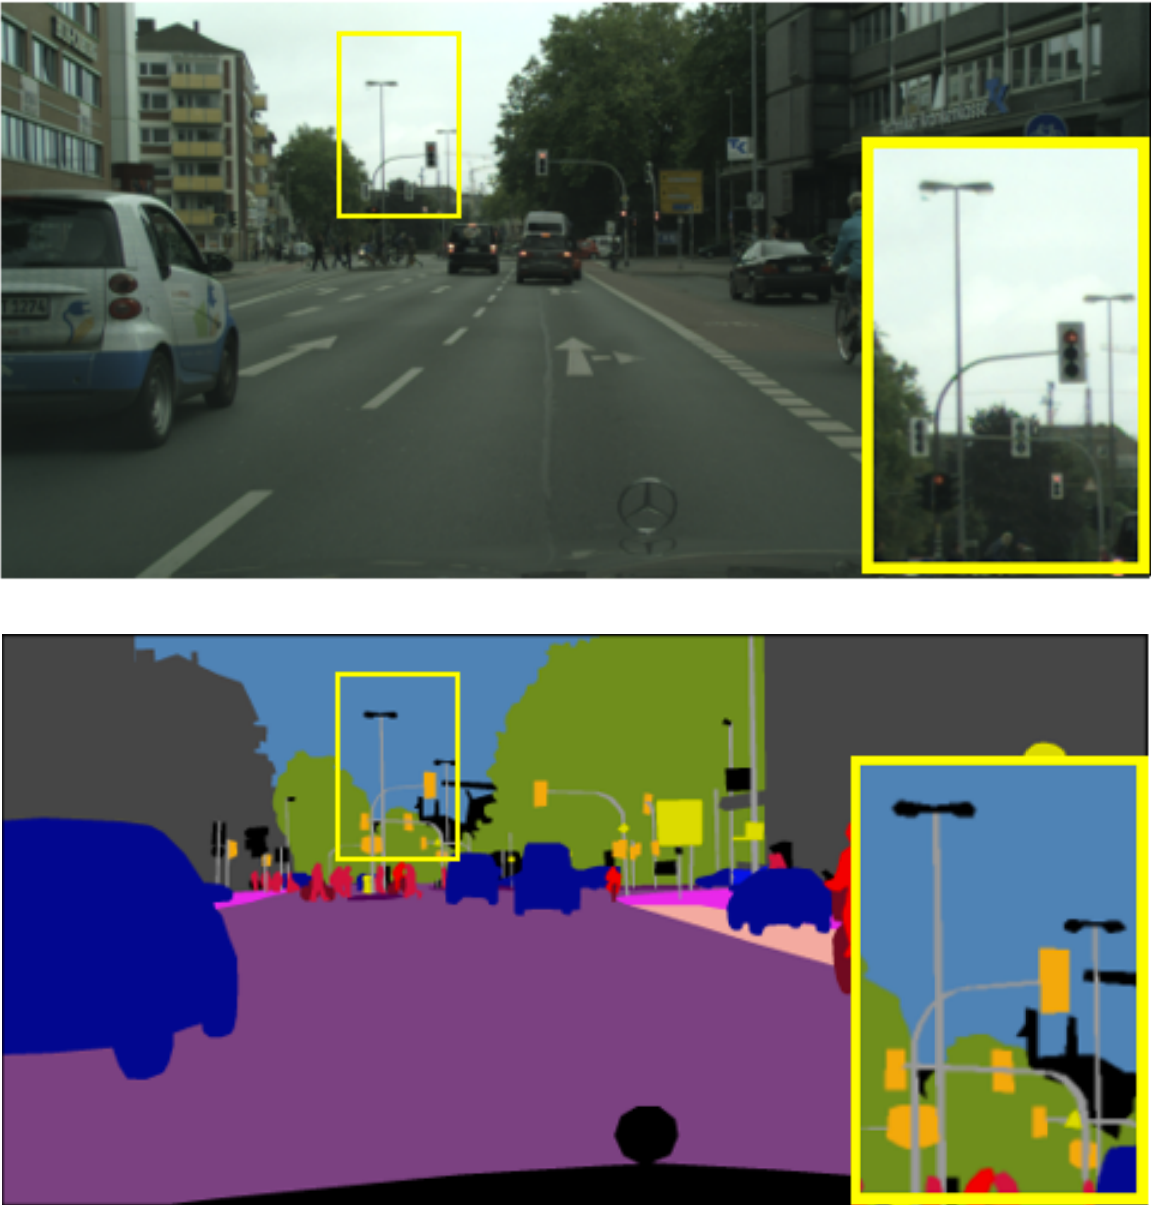
\includegraphics[scale=0.4]{figures/motivation/image-analysis/segmentation-cars.png} &
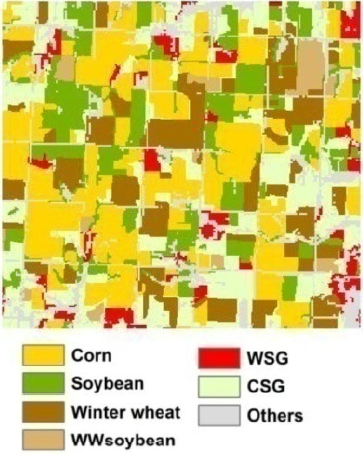
\includegraphics[scale=0.4]{figures/motivation/image-analysis/segmentation-crops.png}\\
\mycite{li2019gff} & \mycite{li2015object}
\end{tabular}}%
\only<3>{
\center
\begin{tabular}{cc}
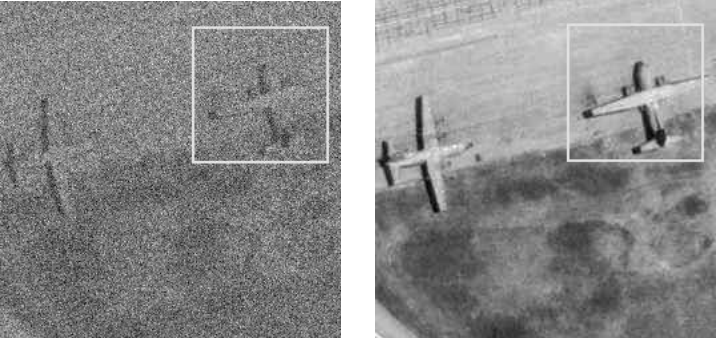
\includegraphics[scale=0.44]{figures/motivation/image-analysis/denoising-airplane.png} &
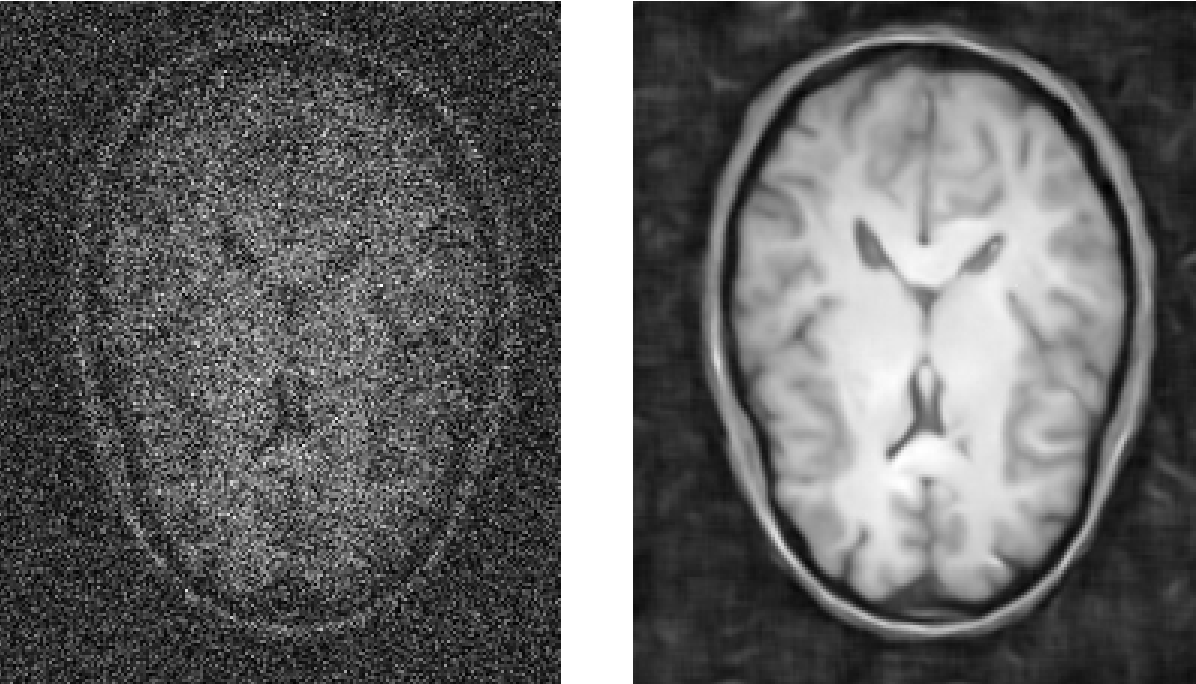
\includegraphics[scale=0.22]{figures/motivation/image-analysis/denoising-mri.png} \\
\mycite{xu2018deep} & \mycite{jiang2018denoising}
\end{tabular}}%
\only<4>{
\center
\begin{tabular}{cc}
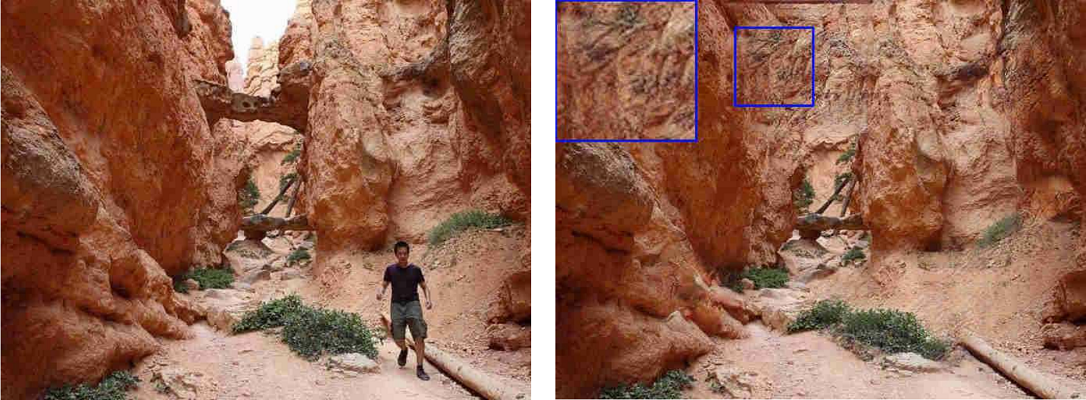
\includegraphics[scale=0.3]{figures/motivation/image-analysis/inpainting-man.png} &
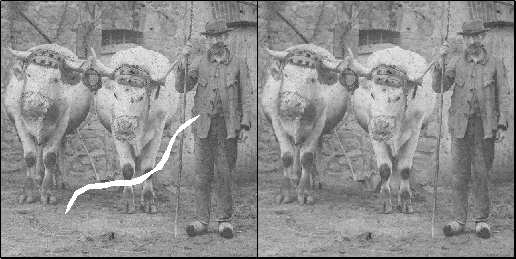
\includegraphics[scale=0.24]{figures/motivation/image-analysis/inpainting-picture.png} \\
\mycite{yu2018generative} &  \mycite{masnou98inpainting}
\end{tabular}}%
\only<5->{
\begin{tabular}{p{0.6\textwidth}p{0.2\textwidth}}
\textbf{Segmentation:} $\mathcal{I}^{\star} = \argmin_{\mathcal{I}} E_{seg}(\mathcal{I},f_{\vec{I}}).$ & \raisebox{-.5\height}{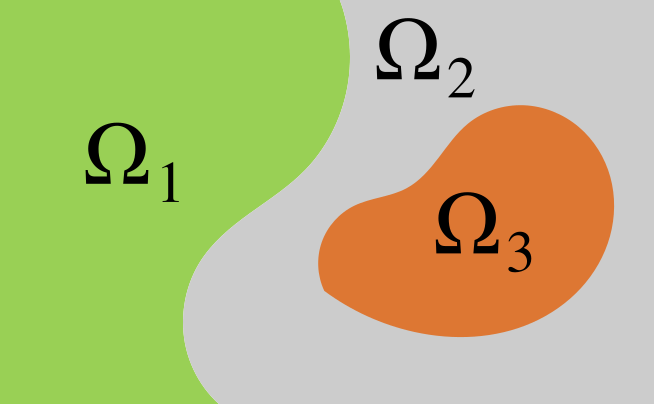
\includegraphics[scale=0.24]{figures/motivation/image-analysis/segmentation-stylised.png}}\\[2em]
\textbf{Denoising:} $f_{\widehat{\vec{I}}} = \argmin_f E_{den}(f,f_{\vec{\widetilde{I}}}).$ & \raisebox{-.5\height}{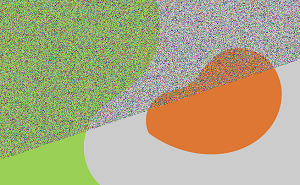
\includegraphics[scale=0.24]{figures/motivation/image-analysis/denoising-stylised.png}}\\[2em]
\textbf{Inpainting:} $f_{\vec{\widehat{I}}} = \argmin_f E_{inp}(f,f_{\widetilde{\vec{I}}}).$ & \raisebox{-.5\height}{
\includegraphics[scale=0.24]{figures/motivation/image-analysis/inpainting-stylised.png}}
\end{tabular}}
\end{minipage}
%6
%
\begin{minipage}[t][0.27\textheight][t]{\textwidth}
\only<5->{We focused on \emph{variational approaches} to solve these problems.}

\only<6->{
Energies are defined by terms that guides the optimization towards solution with special properties e.g.,
\begin{itemize}
	\item{ \emph{Data fidelity}. The solution should not differ much from the input. }
	\item{ \emph{Spatial coherence}. Images are composed of regions with low variability in color. }
\end{itemize}
}
\end{minipage}

\end{frame}







\begin{frame}
{Motivation}
{Geometric priors}
The \emph{Mumford Shah}~(\mycite{mumford89}) is a model for segmentation and denoising.
%
%
\begin{align*}
	\min_{f,\highlight{4}{1-3,5-}{\mathcal{K}}} \alpha \int_{\Omega} \highlight{2}{1,3-}{\norm{ f_{\vec{I}} - f}^2}dx + \beta \int_{\Omega \setminus \highlight{4}{1-3,5-}{\mathcal{K}}} \highlight{3}{1,2,4-}{\norm{ \nabla f}^2} dx + \lambda Per(\highlight{4}{1-3,5-}{\mathcal{K}}).
\end{align*}
%
%
\onslide<5->{
The \emph{ROF}~(\mycite{rudin92}) model uses \emph{total variation} for image denoising.
%
%
\begin{align*}
	\min_{f} \alpha \int_{\Omega} \norm{ f_{\vec{I}} - f}^2dx + \beta \int_{\Omega} \highlight{6}{1-5,7-}{\norm{ \nabla f }}dx.
\end{align*}}
%
%
\onslide<7->{
\begin{itemize}
	\item{A measure of perimeter is present in both models.}
	\item{\emph{Geometric priors} as perimeter, area or curvature are useful due to its flexibility and effect predictability.}
\end{itemize}}
%
%
\vspace{1em}
\onslide<8->{
In this thesis, we are interested in the combined use of \emph{perimeter} and \emph{squared curvature} as geometric priors.}
\end{frame}

\begin{frame}
{Motivation}
{Completion property}
\begin{minipage}[t][0.5\textheight][t]{\textwidth}
\only<1->{
\center
$\min_{ \Omega \in \{\Omega_{c}, \Omega_{d} \} } Perimeter(\Omega).$
}
\only<1>{
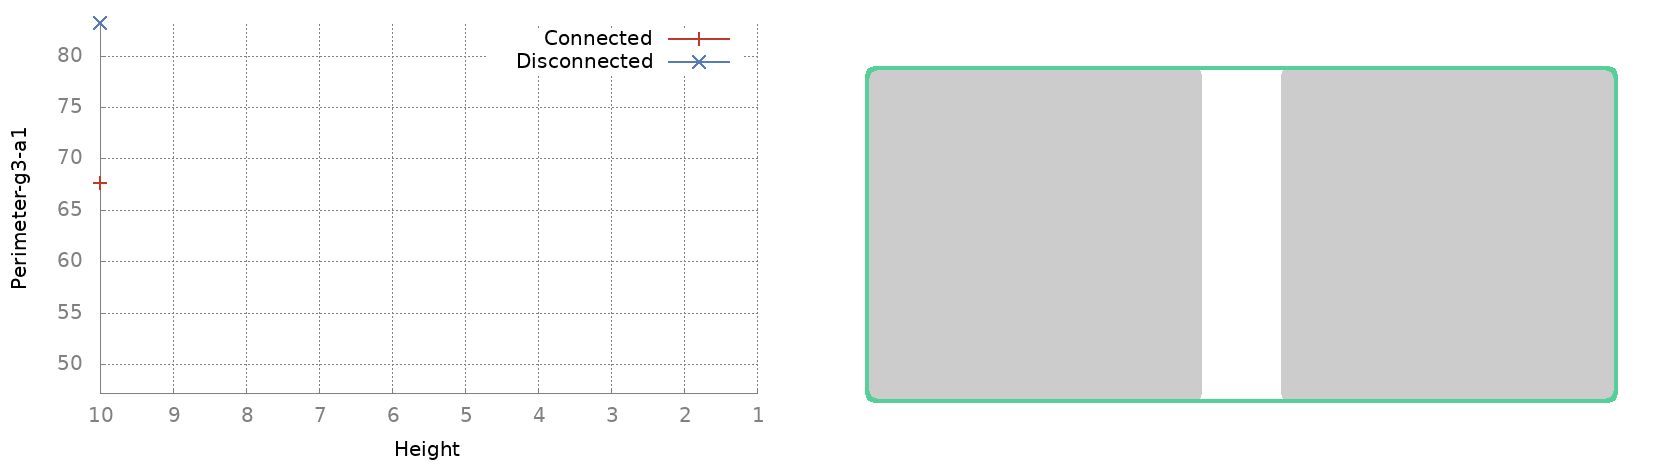
\includegraphics[scale=0.25]{figures/motivation/completion/perimeter-0.png}
}
\only<2>{
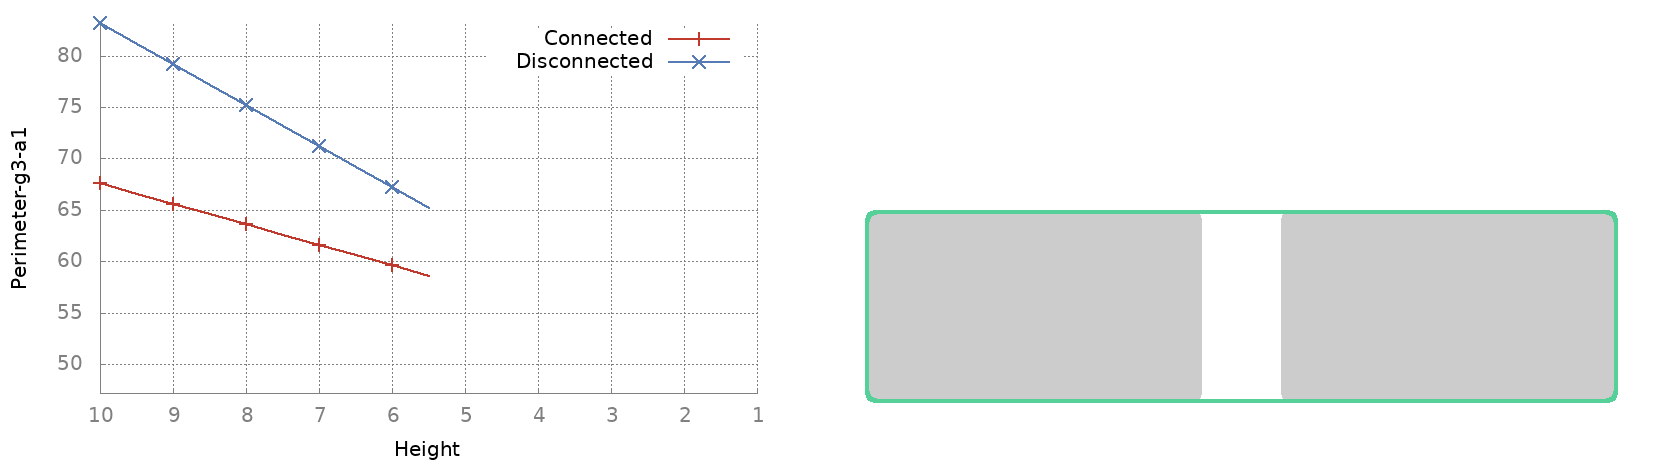
\includegraphics[scale=0.25]{figures/motivation/completion/perimeter-1.png}
}
\only<3>{
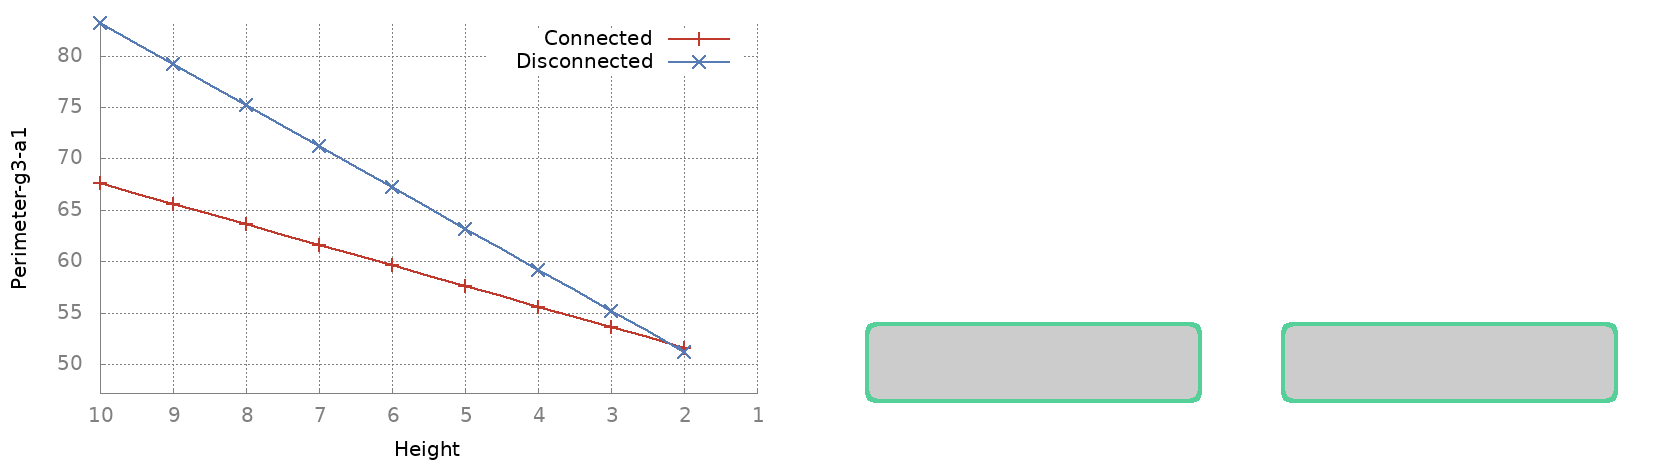
\includegraphics[scale=0.25]{figures/motivation/completion/perimeter-2.png}
}
\only<4->{
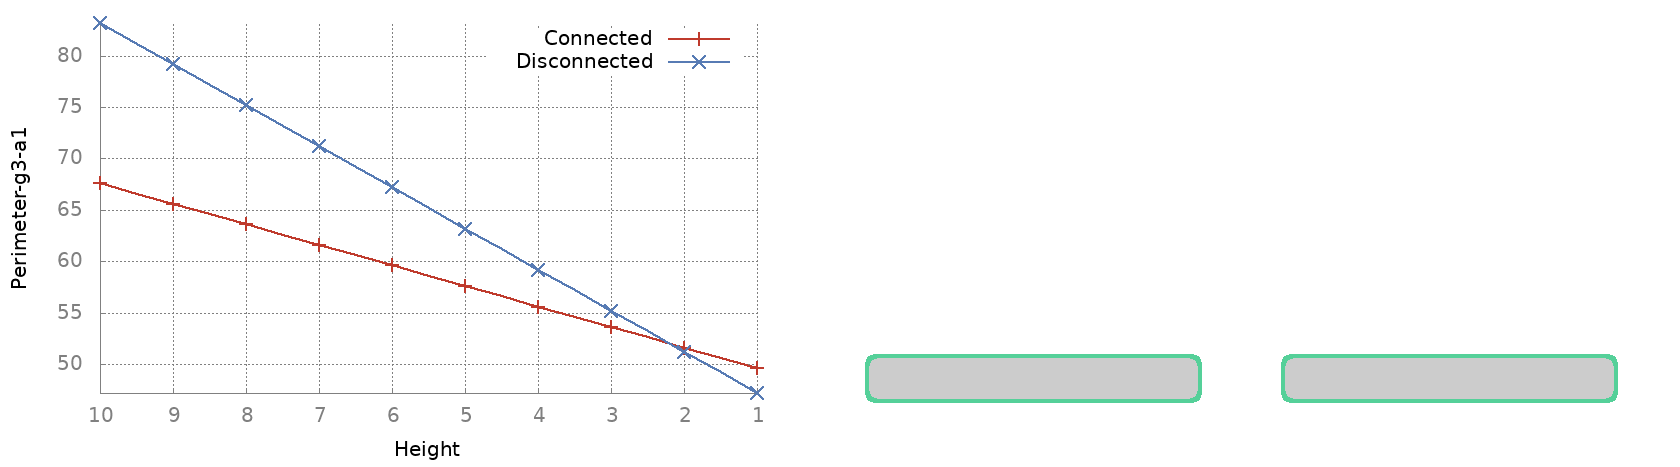
\includegraphics[scale=0.25]{figures/motivation/completion/perimeter-3.png}
}
\end{minipage}
\begin{minipage}[t][0.5\textheight][t]{\textwidth}
\only<5->{
\center
$\min_{ \Omega \in \{\Omega_{c}, \Omega_{d} \} } Perimeter(\Omega) + Squared\;Curvature(\partial \Omega).$}
\only<5>{
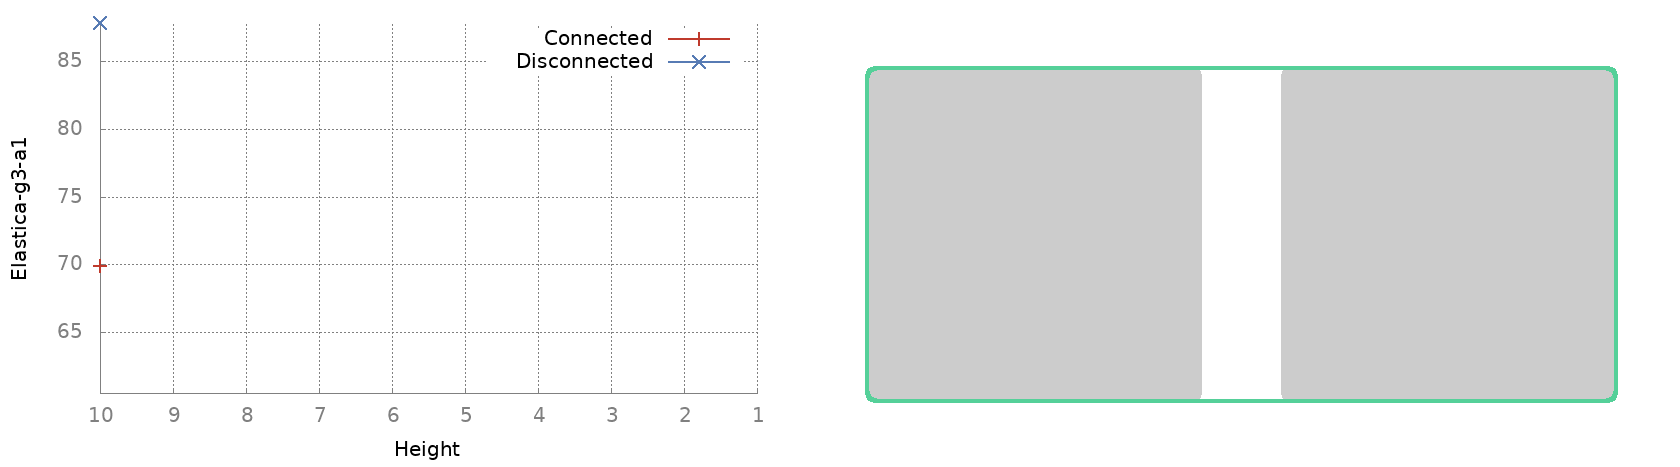
\includegraphics[scale=0.25]{figures/motivation/completion/elastica-0.png}
}
\only<6>{
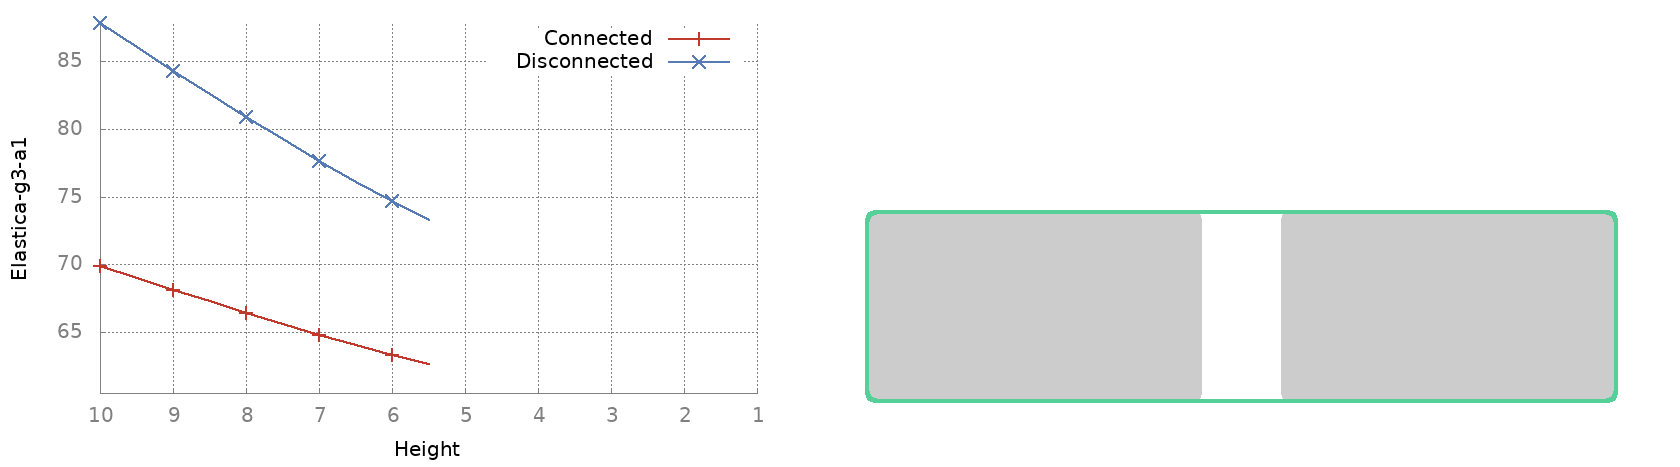
\includegraphics[scale=0.25]{figures/motivation/completion/elastica-1.png}
}
\only<7>{
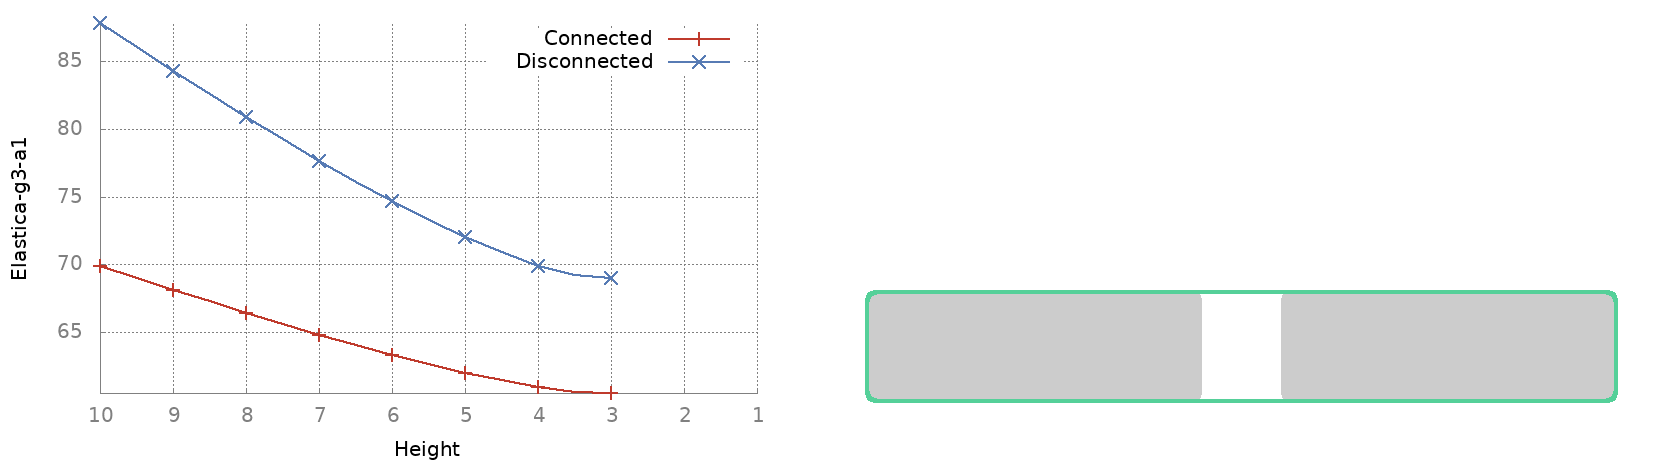
\includegraphics[scale=0.25]{figures/motivation/completion/elastica-2.png}
}
\only<8->{
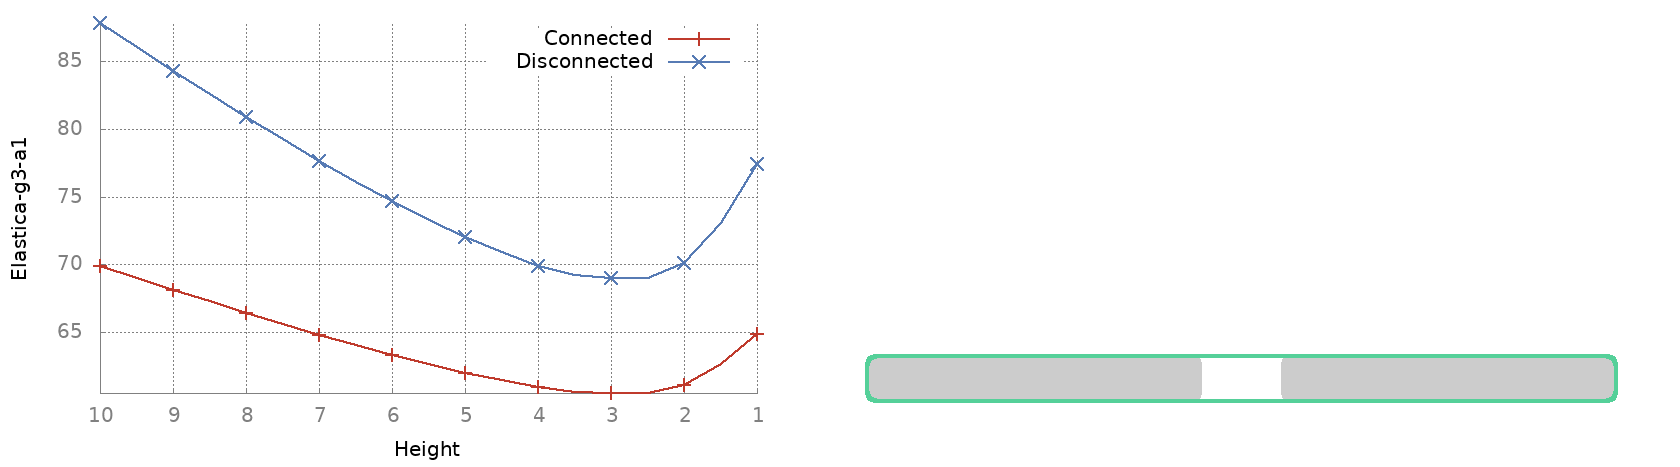
\includegraphics[scale=0.25]{figures/motivation/completion/elastica-3.png}
}
\end{minipage}
\end{frame}

\begin{frame}
{Motivation}
{Completion property}
\begin{minipage}[t][0.5\textheight][t]{\textwidth}
\only<1->{
\center
$\min_{ \Omega \in \{\Omega_{c}, \Omega_{d} \} } Perimeter(\Omega) + Squared\;Curvature(\partial \Omega).$}
\only<1>{
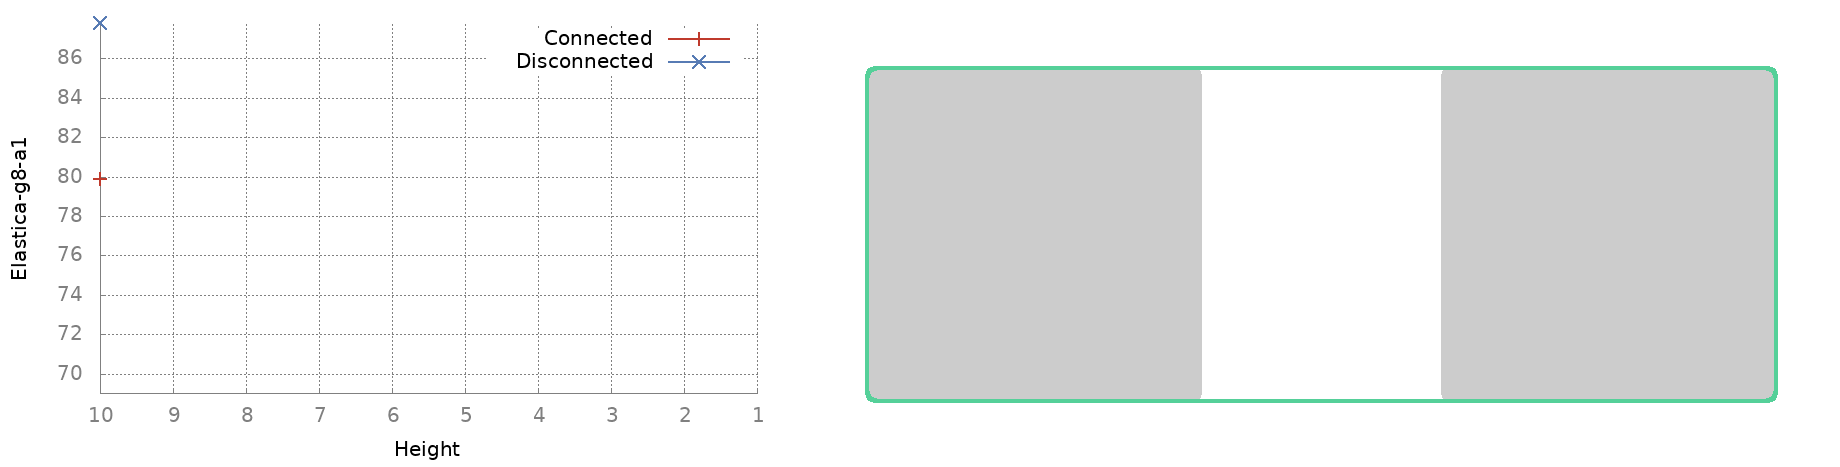
\includegraphics[scale=0.22]{figures/motivation/completion/elastica-g8a1-0.png}
}
\only<2>{
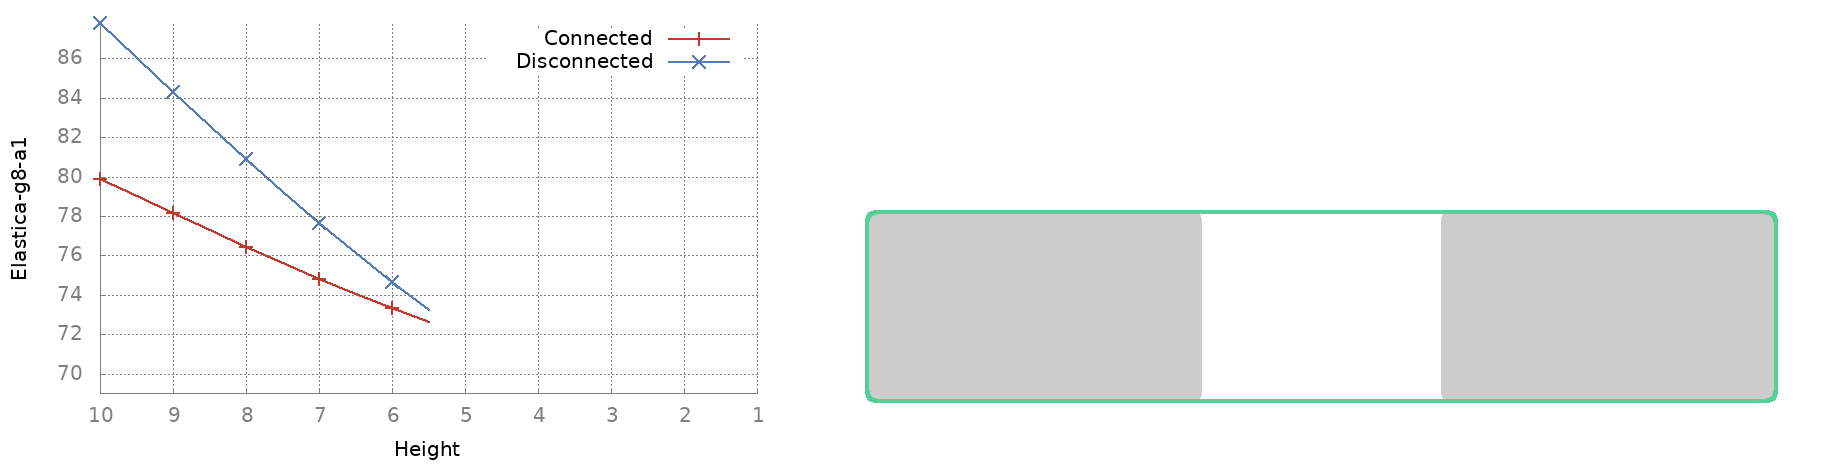
\includegraphics[scale=0.22]{figures/motivation/completion/elastica-g8a1-1.png}
}
\only<3>{
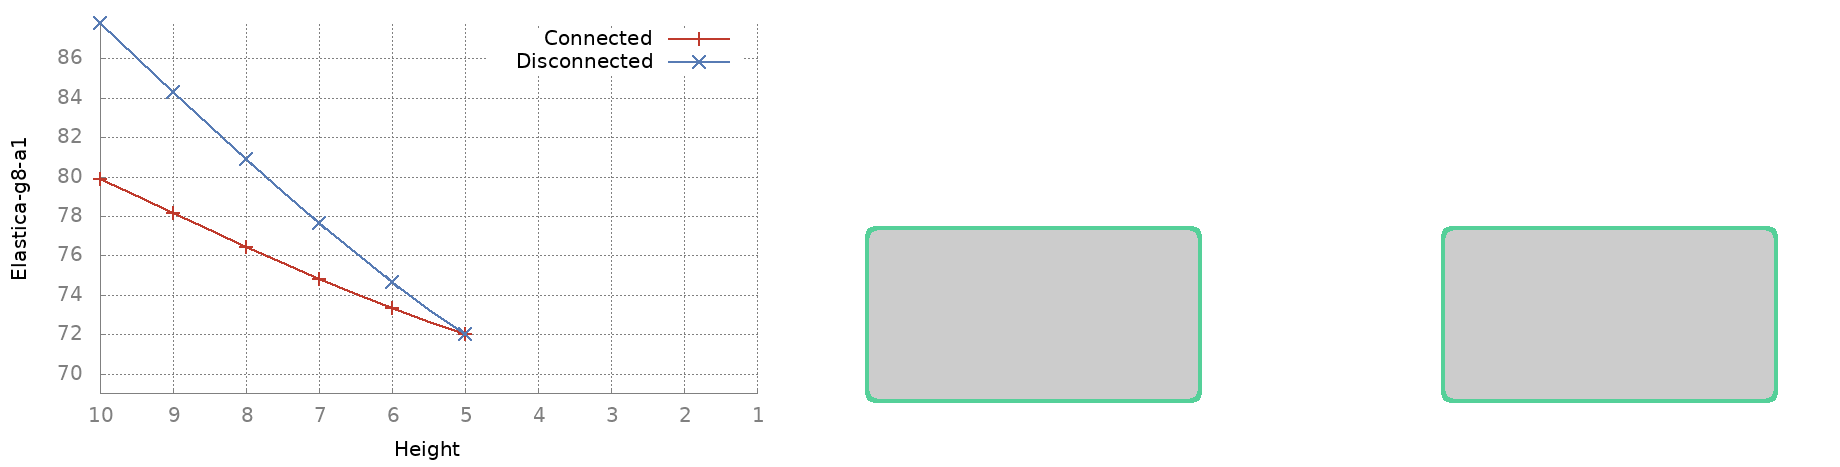
\includegraphics[scale=0.22]{figures/motivation/completion/elastica-g8a1-2.png}
}
\only<4>{
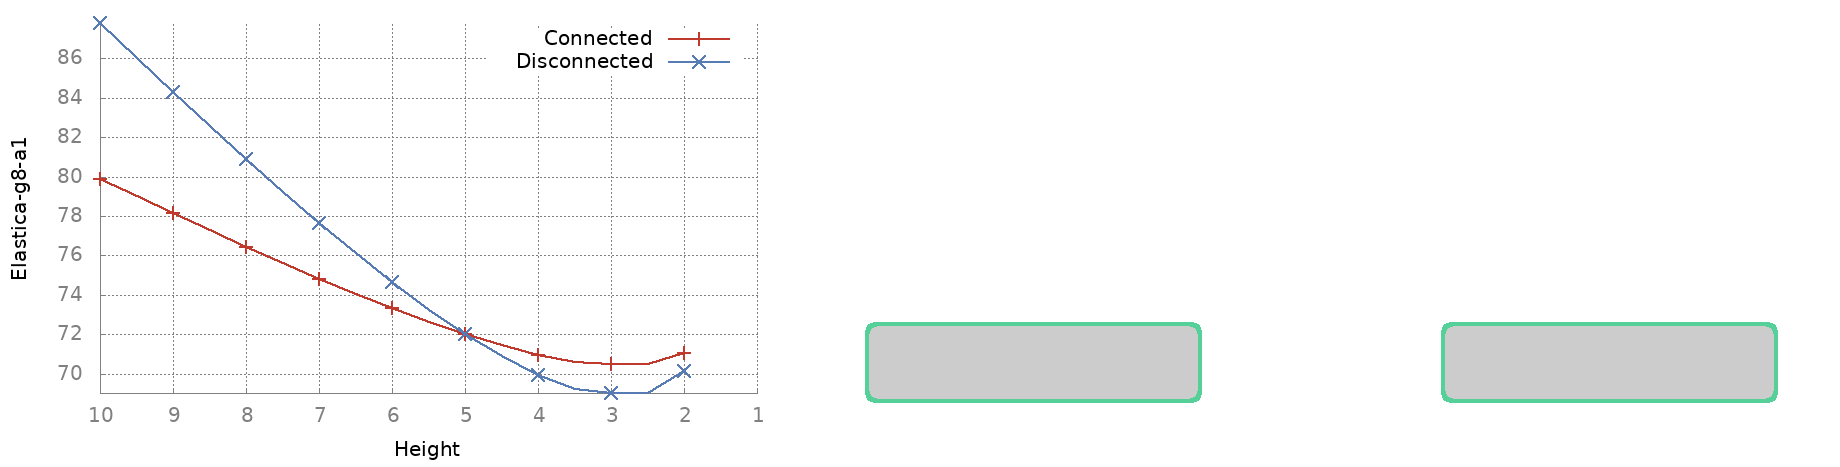
\includegraphics[scale=0.22]{figures/motivation/completion/elastica-g8a1-3.png}
}
\only<5->{
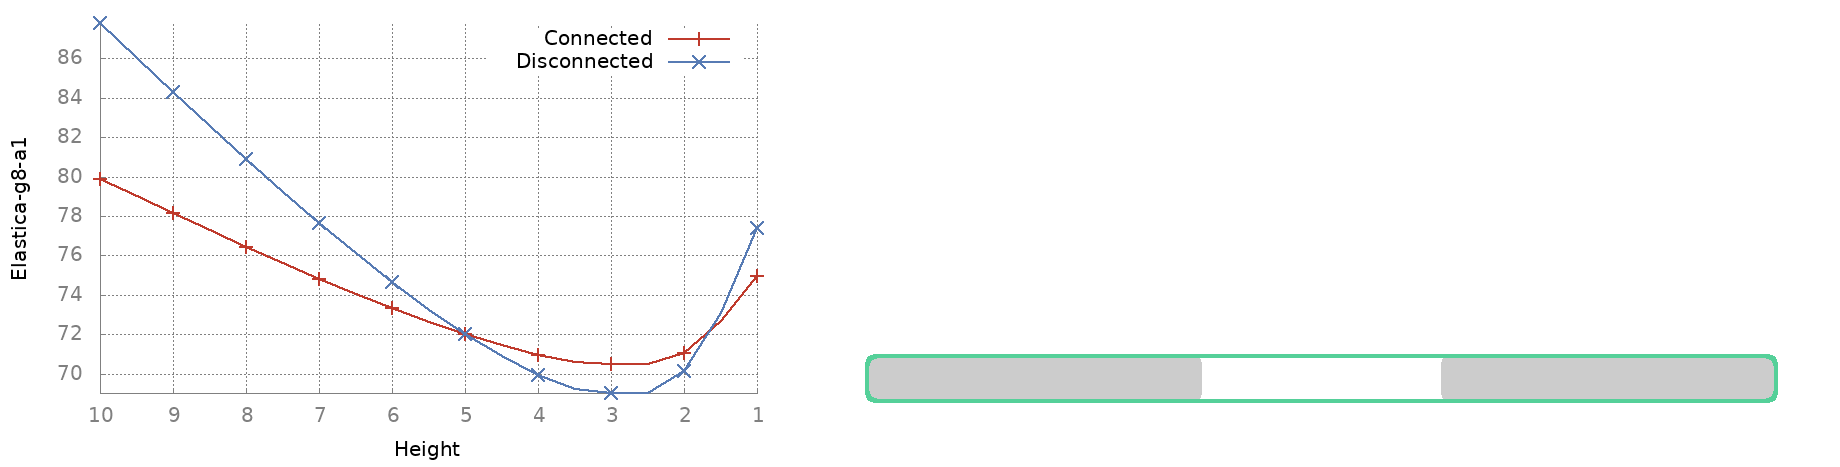
\includegraphics[scale=0.22]{figures/motivation/completion/elastica-g8a1-4.png}
}
\end{minipage}
\begin{minipage}[t][0.5\textheight][t]{\textwidth}
\only<6-9>{
\center
$\min_{ \Omega \in \{\Omega_{c}, \Omega_{d} \} } \frac{1}{2}Perimeter(\Omega) + Squared\;Curvature(\partial \Omega).$}
\only<10->{
\center
\color{highlightcolor} $\min_{ \Omega \in \{\Omega_{c}, \Omega_{d} \} } \int_{\partial \Omega}{ \alpha + \beta \kappa ^2ds}. \quad - \quad \text{The elastica energy}$}
\only<6>{
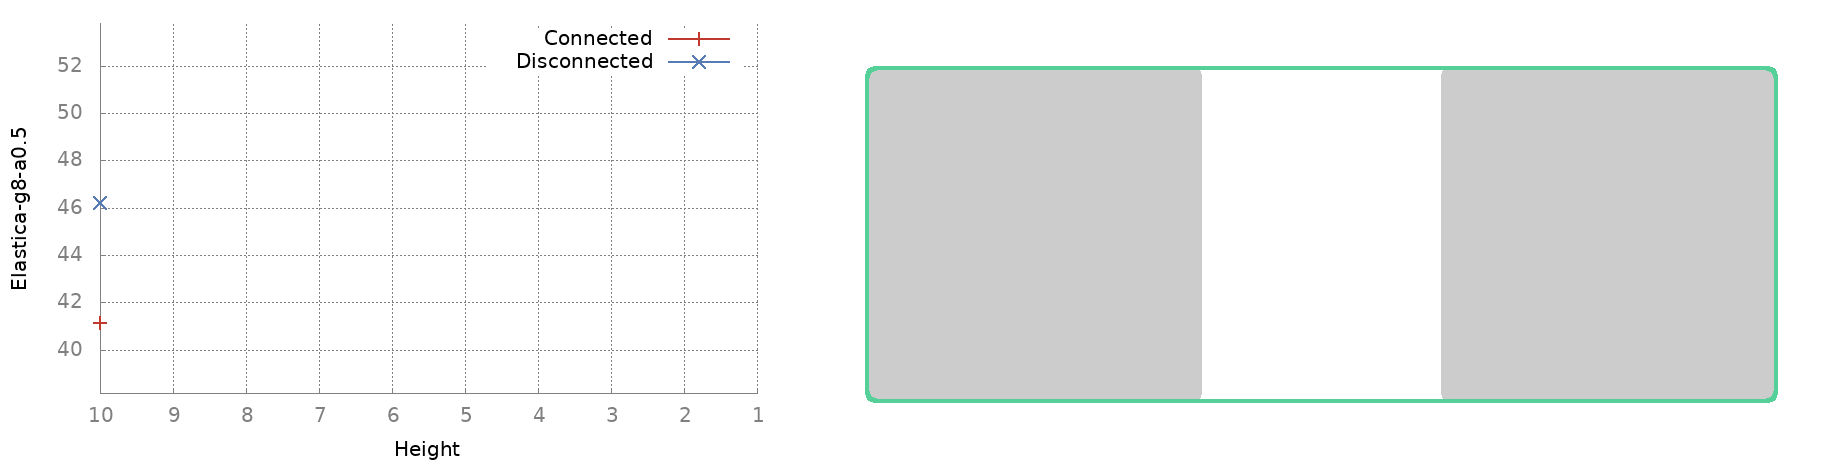
\includegraphics[scale=0.22]{figures/motivation/completion/elastica-g8a05-0.png}
}
\only<7>{
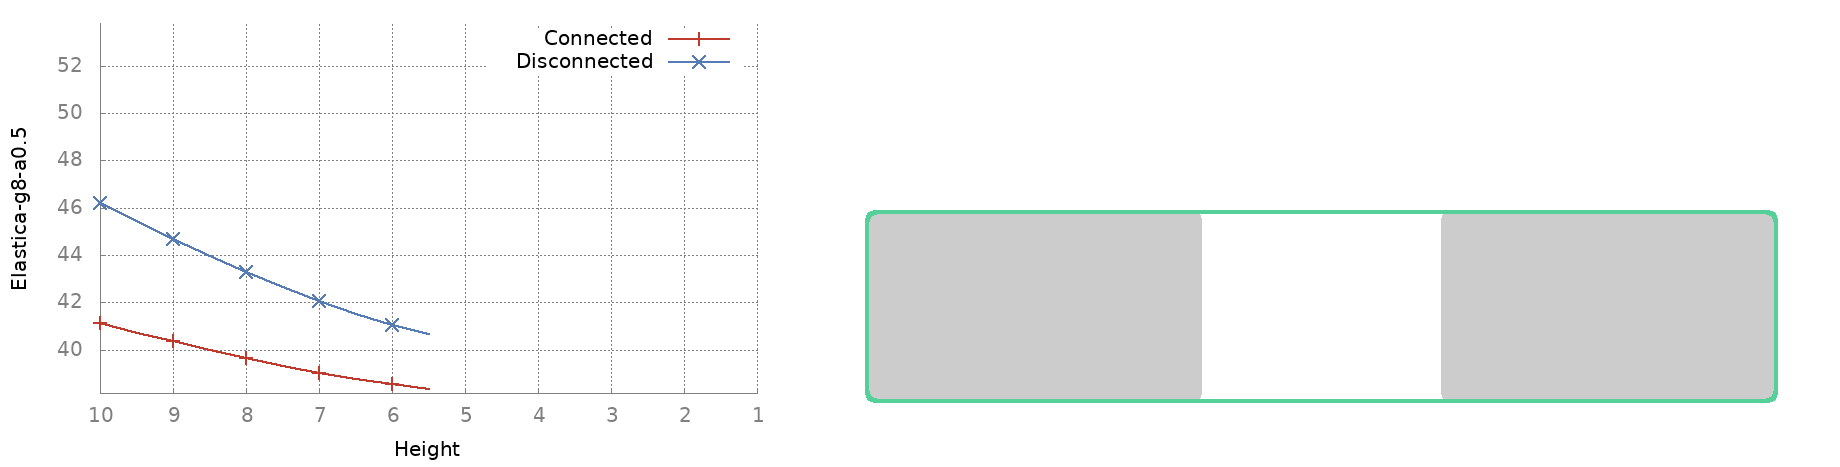
\includegraphics[scale=0.22]{figures/motivation/completion/elastica-g8a05-1.png}
}
\only<8>{
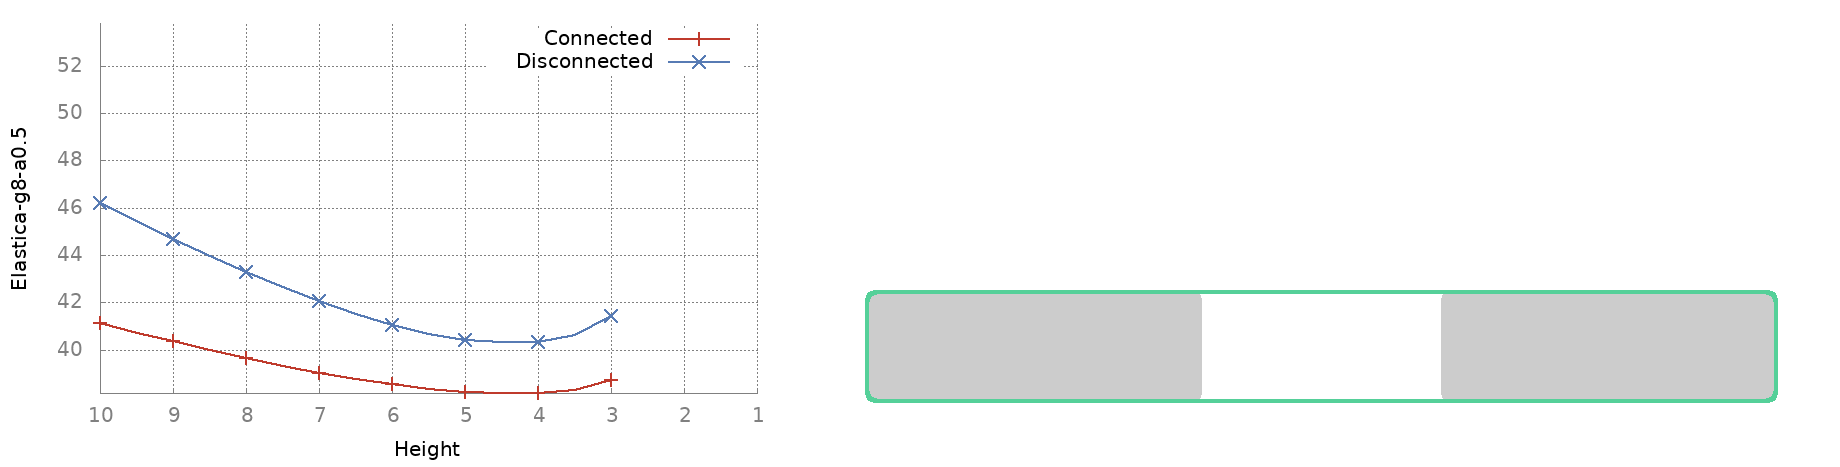
\includegraphics[scale=0.22]{figures/motivation/completion/elastica-g8a05-2.png}
}
\only<9->{
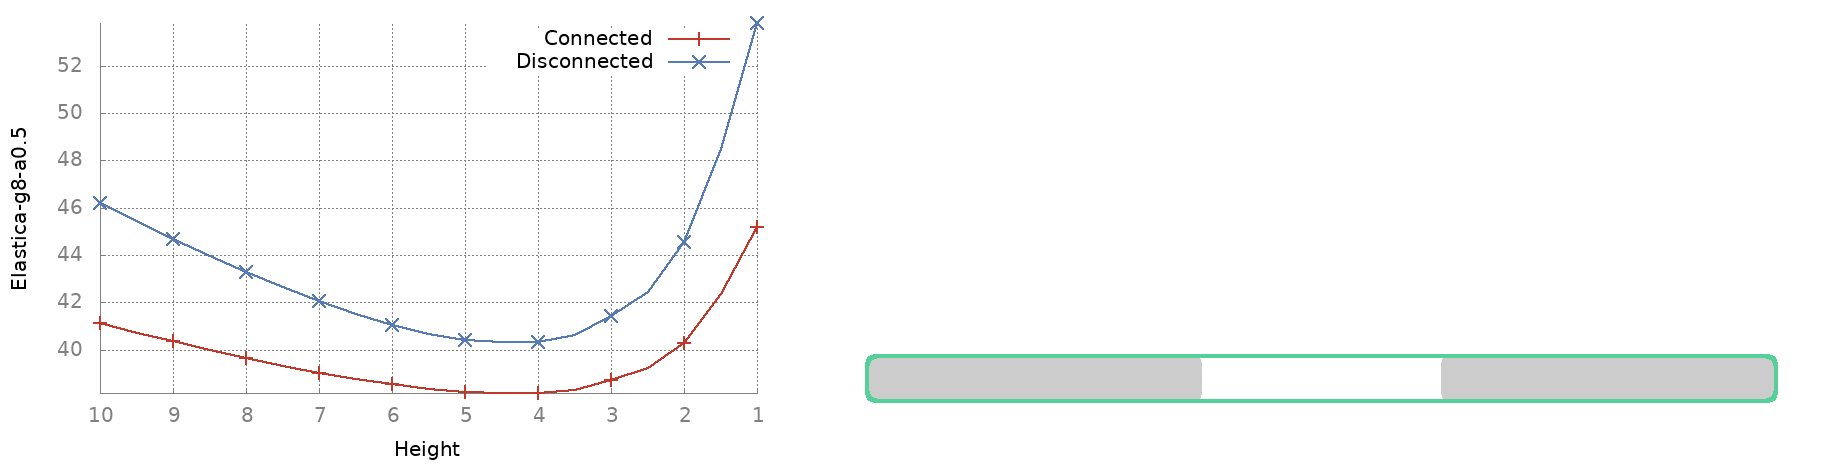
\includegraphics[scale=0.22]{figures/motivation/completion/elastica-g8a05-3.png}
}
\onslide<11>{
	\begin{figure}
	\begin{tikzpicture}[overlay, remember picture] 
	\node at (current page.center) 
	    [
	    anchor=east,
	    xshift=-10mm,
	    yshift=0mm
	    ] 
	{
	
	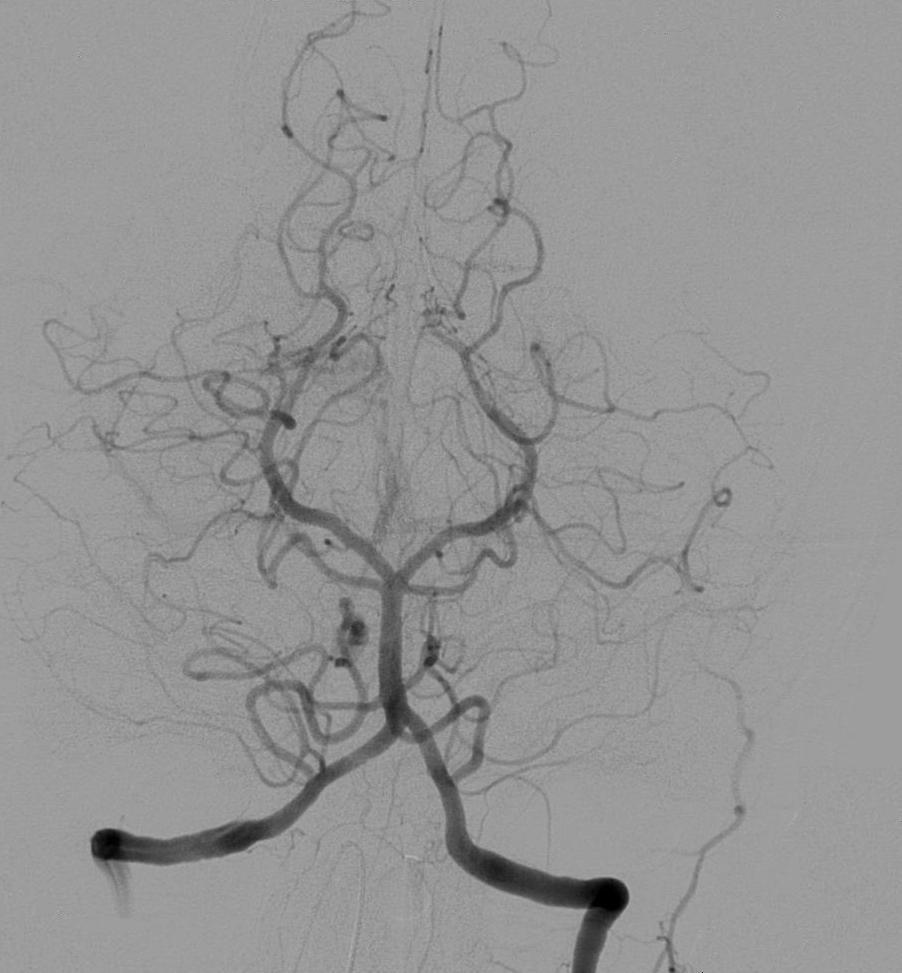
\includegraphics[scale=0.16]{figures/motivation/completion/angiogram.jpg}
		
	};
	\node at (current page.center) 
	    [
	    anchor=west,
	    xshift=-10mm,
	    yshift=0mm
	    ] 
	{
	
	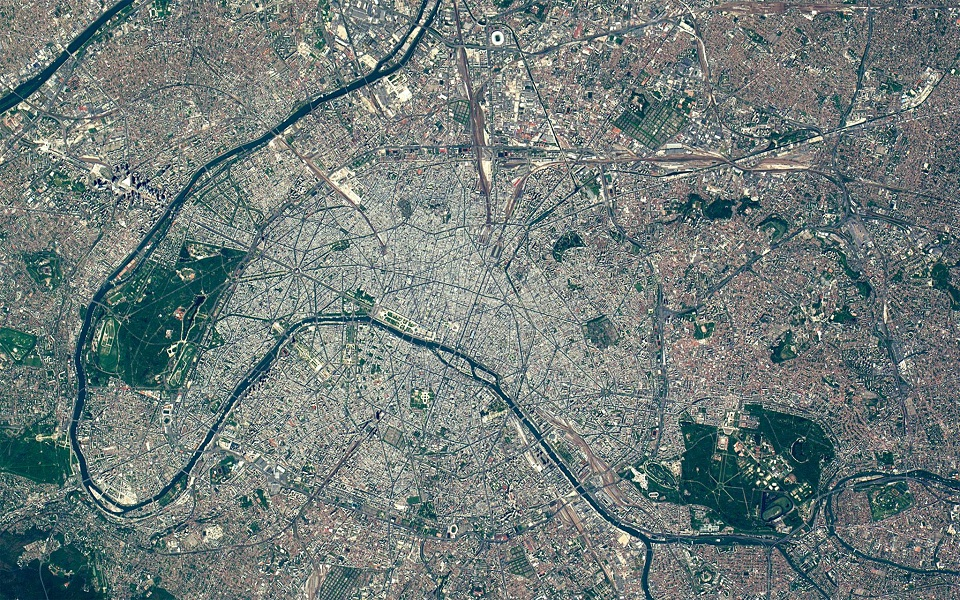
\includegraphics[scale=0.35]{figures/motivation/completion/paris-satellite-road.jpg}
		
	};	
	\end{tikzpicture}	
	\end{figure}	
	}	
\end{minipage}
\end{frame}

\begin{frame}
{Motivation}
{State-of-the-art}
\small
\textbf{Continuous setting}: Define the energy over the whole domain and minimize the elastica with respect the level-curves~(\mycite{chan02elasticainpainting}).
%
\begin{align*}
\int_{\Omega}{ \left(\alpha + \beta \nabla \cdot \left(\frac{\nabla f_{\vec{I}}}{\norm{\nabla f_{\vec{I}} }}\right) ^2 \right)\norm{\nabla f_{\vec{I}} }d\Omega}.
\end{align*}
%
\pause
\begin{itemize}
\item{Numerical instability: Fourth-order Euler-Lagrange equation.}
\item{Susceptible to bad local minimum.}
\end{itemize}
%
\pause
\vspace{0.5em}
\textbf{Discrete setting}:
\vspace{-1em}
\setlength\tabcolsep{3pt}
\begin{center}
\renewcommand{\arraystretch}{0.25}
\begin{tabular}{p{0.4\textwidth}p{0.6\textwidth}}
T-junctions matching & \multirow{2}{0.6\textwidth}{\footnotesize Fast algorithm, but limited to absolute value of curvature (polygonal solutions) and inpainting application.} \\
\mycite{masnou98inpainting} &\pause\\[3em]
Linear programming & \multirow{2}{0.6\textwidth}{\footnotesize Global formulation, but prohibitive running times even for small (thus unprecise) neighborhoods. Not suitable for digital sets.} \\
\mycite{schoenemann09linear} &\pause\\[3em]
Triple cliques & \multirow{2}{0.6\textwidth}{\footnotesize Global formulation, quadratic non-submodular energy. Limited precision due combinatorial explosion.} \\
\mycite{nieuwenhuis14efficient} &
\end{tabular}
\end{center}
\end{frame}

\begin{frame}
{Motivation}
{Goals}

Models based on the minimization of the elastica energy

\center
\begin{tabular}{lcc|c|}
& Continuous & Discrete & \textbf{Digital} \\
\hline
Numerical instability & \negative{Yes} & \positive{No} & \positive{No} \\
Suitable for digital sets & \negative{No} & \negative{No} & \positive{Yes} \\
Rounding issues & \negative{Yes} & \positive{No} & \positive{No} \\
Global formulation & \positive{Yes} & \positive{Yes} & \negative{No} \\
Contour completion & \negative{Partial} & \negative{Partial} & \positive{Extended} \\
Global optimum (Free elastica) & \negative{-} & \negative{-} & \positive{Yes}
\end{tabular}

%\vspace{2em}
%
%\begin{itemize}
%\item{Can we define an elastica-based model for image analysis using multigrid convergent estimators? \only<4>{\positive{Yes!}}} \pause
%\item{Can we recover the completion property of elastica? \only<4>{\positive{Yes!}}} \pause
%\item{Can we escape bad local minima? \only<4>{\positive{Yes!}}}
%\end{itemize}

\end{frame}



\begin{frame}
	{Presentation plan}

\begin{enumerate}
	{\transparent{0.4}%
	\item{Motivation}
	\begin{itemize}
		\item{Image analysis and Geometric priors}
		\item{Elastica and completion property}		
		\item{State-of-art}				
		\item{Multigrid convergent estimators}						
	\end{itemize}}
	\vspace{1em}
	\item{Contribution}
	\begin{itemize}
		\item{A combinatorial model for elastica}
		\item{A quadratic non-submodular formulation for elastica}	
		\item{Elastica minimization via graph-cuts}	
	\end{itemize}
	\vspace{1em}
	\item{Conclusion and perspectives}
\end{enumerate}

\end{frame}

\section{Combinatorial Elastica}

\begin{frame}
	{Combinatorial Elastica}	

\end{frame}
\section{Non-submodular elastica}

\begin{frame}
\begin{center}
\huge
A quadratic non-submodular formulation for elastica
\end{center}
\end{frame}

\begin{frame}
{Non-submodular elastica}	
{Local models and completion effect}

\begin{minipage}[t][0.7\textheight][t]{1\textwidth}
\center

The completion effect can be difficult to recover in local approaches.\vspace{1em}

\only<2>{

\includegraphics[scale=0.5]{figures/non-submodular-elastica/completion/completion-1.png}
}%
\only<3>{
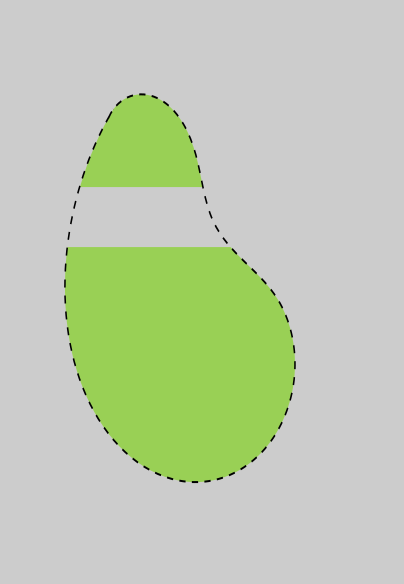
\includegraphics[scale=0.5]{figures/non-submodular-elastica/completion/completion-2.png}
}%
\only<4->{
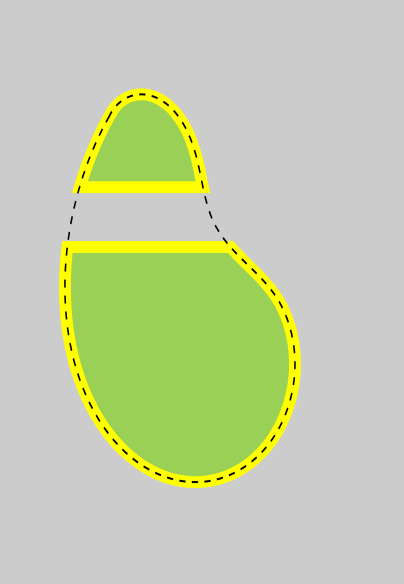
\includegraphics[scale=0.5]{figures/non-submodular-elastica/completion/completion-3.png}
}%
\vspace{1em}

\onslide<5->{However, a global optimization carries its own bag of issues.}
\end{minipage}

\end{frame}

\begin{frame}
	{Non-submodular elastica}	
	{Difficulties with a global model}
\begin{minipage}[t][0.6\textheight][t]{1\textwidth}
\begin{minipage}{0.35\textwidth}
\only<1>{
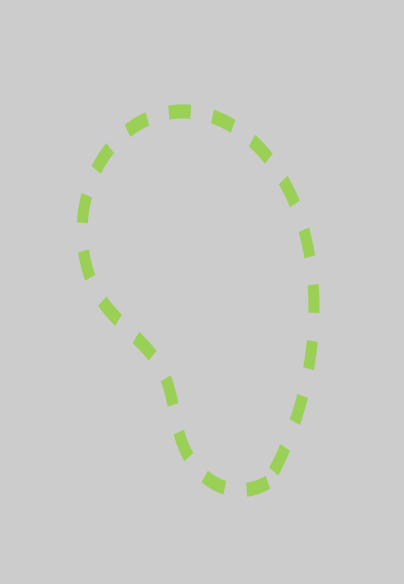
\includegraphics[scale=0.5]{figures/non-submodular-elastica/global/issues-2.png}
}
\only<2>{
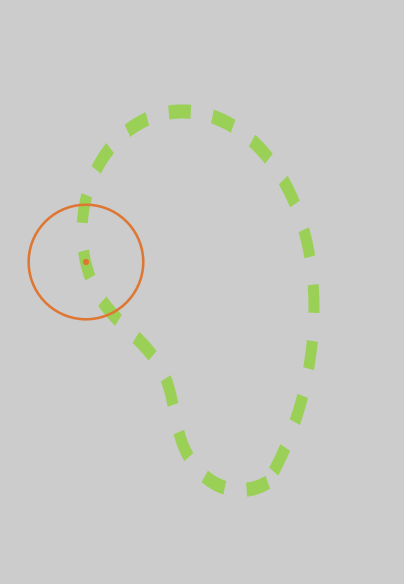
\includegraphics[scale=0.5]{figures/non-submodular-elastica/global/issues-3.png}
}
\only<3>{
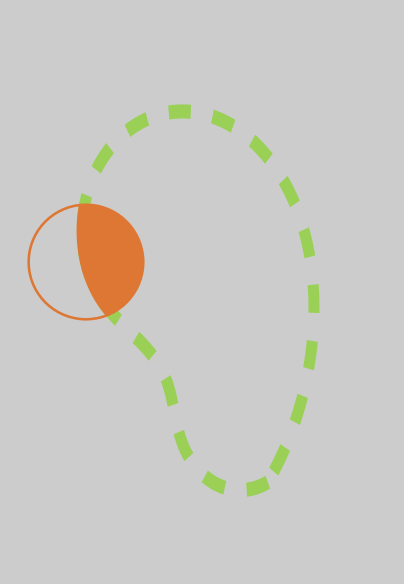
\includegraphics[scale=0.5]{figures/non-submodular-elastica/global/issues-4.png}
}
\only<4->{
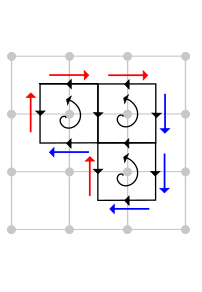
\includegraphics[scale=1]{figures/non-submodular-elastica/global/topological-constraints.png}
}
\end{minipage}
%
%
\begin{minipage}{0.64\textwidth}
\onslide<2->{
\begin{itemize}
	\item{Center of the estimation disk}
	\onslide<3->{\item{Pixel counting and estimation of curvature squared}}
	\onslide<4->{\item{Topological constraints}}	
	\onslide<5->{\item{Third order non-convex binary}}		
	\onslide<6->{\item{Level 1 linearization: non semi-definite positive matrix}}
	\onslide<7->{\item{Level 2 linearization: $O(m^3)$ variables}}
\end{itemize}}
\end{minipage}	
\end{minipage}
%
%
\begin{minipage}[t][0.25\textheight][t]{1\textwidth}
\only<2>{
\begin{align*}
	\sum_{\ell_i \in \mathcal{L}}{ \vec{y}_i \left(\; \alpha + \beta \hat{\kappa}_{r}^2(D,\ell_i) \; \right)}\\\nonumber
\end{align*}}
\only<3>{
\begin{align*}
&\sum_{\ell_i \in \mathcal{L}}{ \vec{y}_i \left(\; \alpha + \frac{9}{r^6}\beta \big(c^2 - 2c\vec{A}_i^T\vec{x} + \vec{x}^T\vec{A}_i\vec{A}_i^T\vec{x}\big)\right)}\\
&\text{subject to} \quad \vec{x} \in \{0,1\}^m, \vec{y} \in \{0,1\}^n.
\end{align*}}
\only<4->{
\begin{align*}
&\sum_{\ell_i \in \mathcal{L}}{ \vec{y}_i \left(\; \alpha + \frac{9}{r^6}\beta \big(c^2 - 2c\vec{A}_i^T\vec{x} + \vec{x}^T\vec{A}_i\vec{A}_i^T\vec{x}\big)\right)}\\
&\text{subject to} \quad \vec{x} \in \{0,1\}^m, \vec{y} \in \{0,1\}^n, T(\vec{x},\vec{y}).
\end{align*}}
\end{minipage}

\end{frame}

\begin{frame}
{Non-submodular elastica}
{Simplification}
\center
$\hat{\kappa}(p) = \frac{3}{r^3}\left( \frac{\pi r^2}{2} - | B_r(p) \cap X | \right )$
\begin{minipage}[t][0.5\textheight]{1\textwidth}
\center
\only<1>{
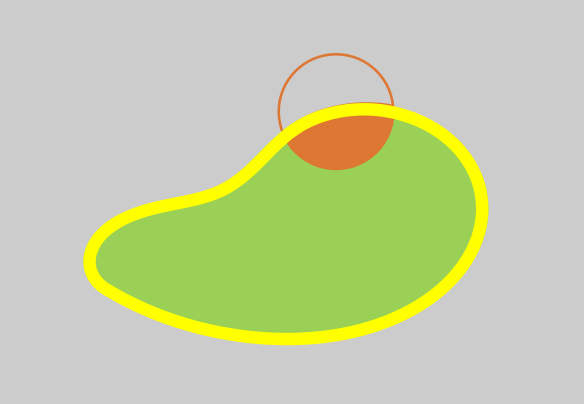
\includegraphics[scale=0.5]{figures/non-submodular-elastica/current-contour.png}}
\only<2>{
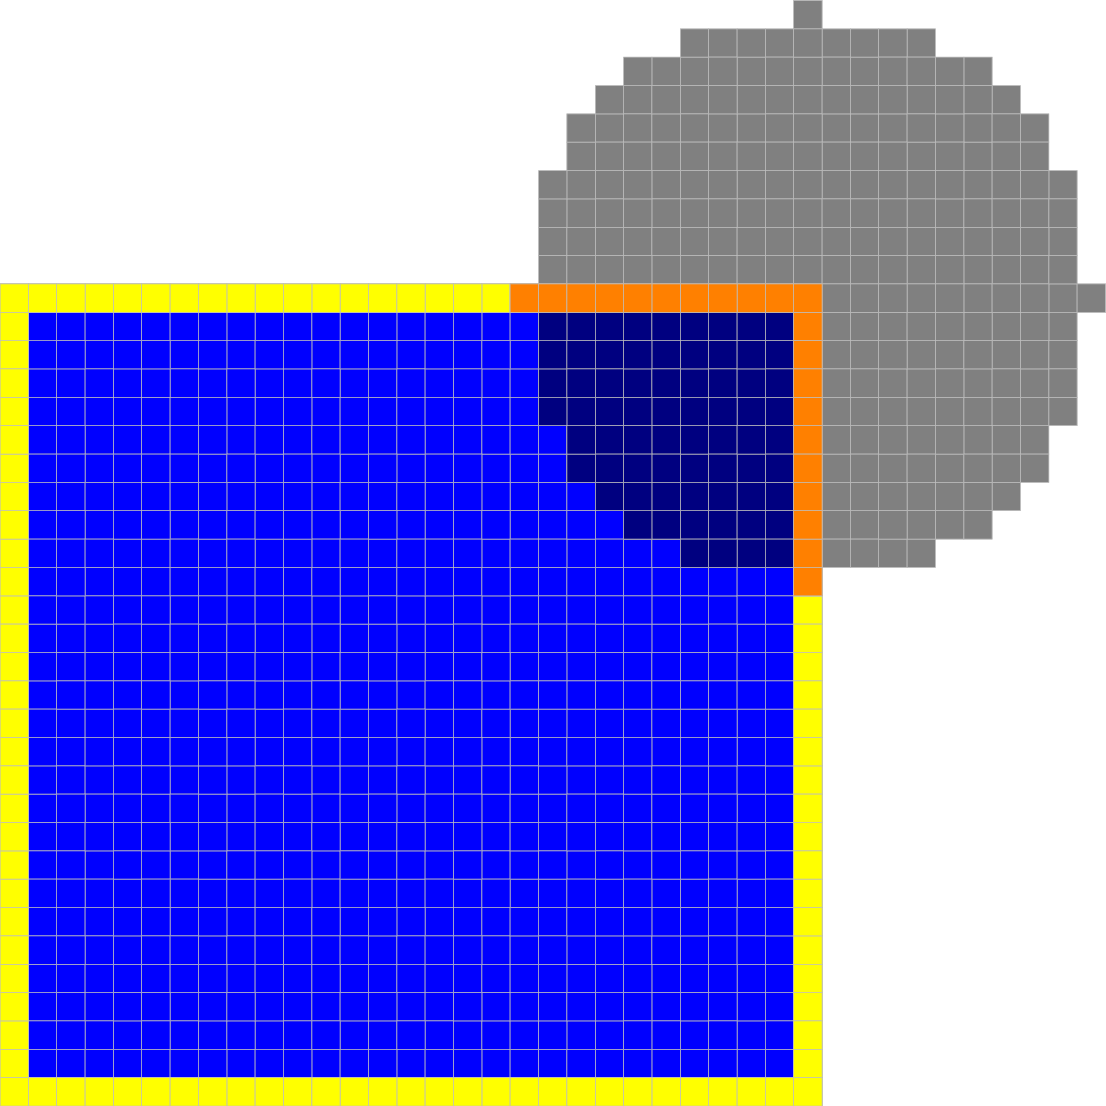
\includegraphics[scale=0.1]{figures/non-submodular-elastica/before-opt.png}\hspace{2em}
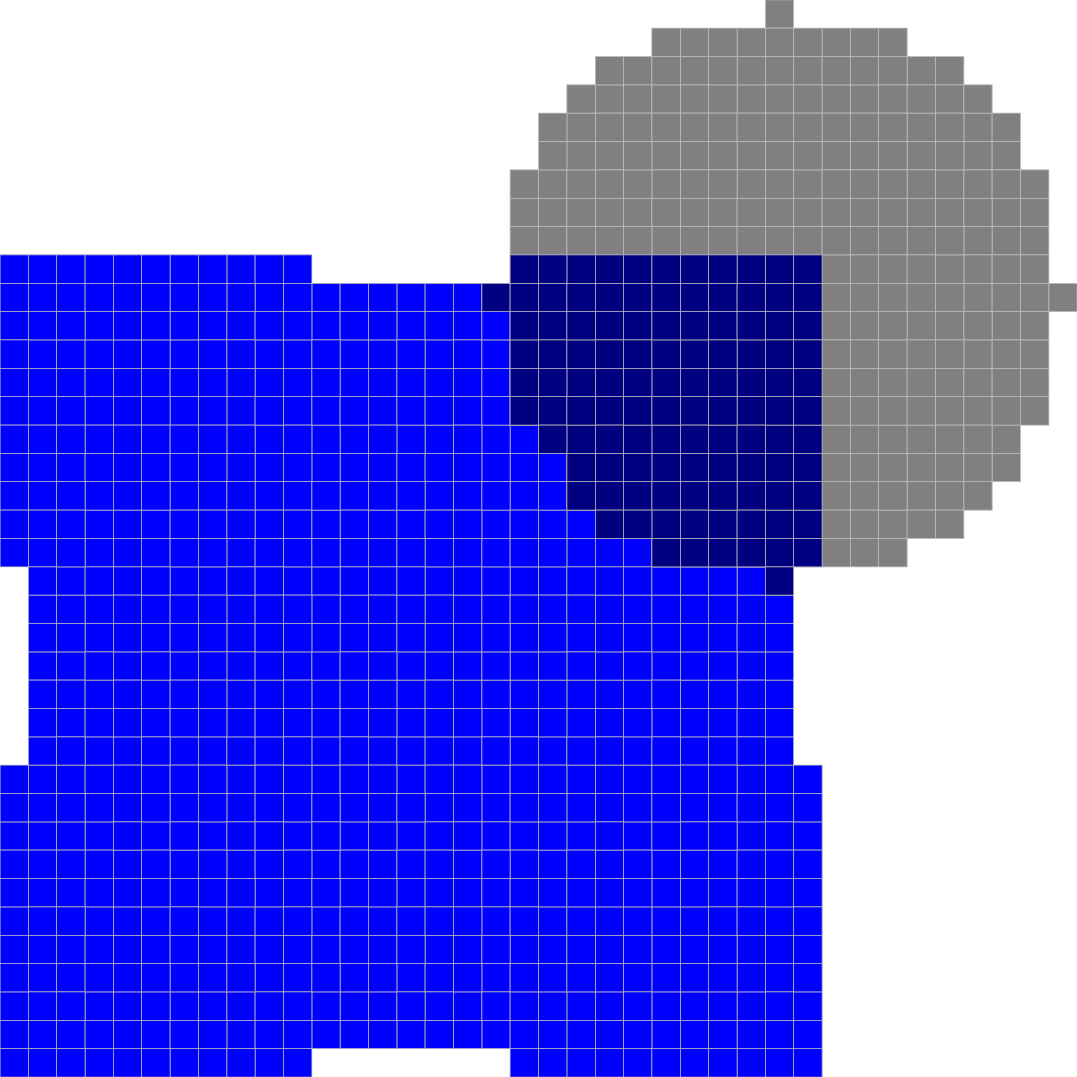
\includegraphics[scale=0.1]{figures/non-submodular-elastica/shape-opt-ball-after.png}}
\end{minipage}

\begin{itemize}
\item{Define the optimization region (yellow) as the inner contour of the shape, denoted $I$.}
\item{Evolve the estimation disks in the current contour.}
\item{Set pixels such that the curvature estimation is reduced.}
\end{itemize}
\end{frame}

\begin{frame}
{Non-submodular elastica}
{Simplification}
\center
$\hat{\kappa}(p) = \frac{3}{r^3}\left( \frac{\pi r^2}{2} - | B_r(p) \cap X | \right )$
\begin{minipage}[t][0.5\textheight]{1\textwidth}
\center
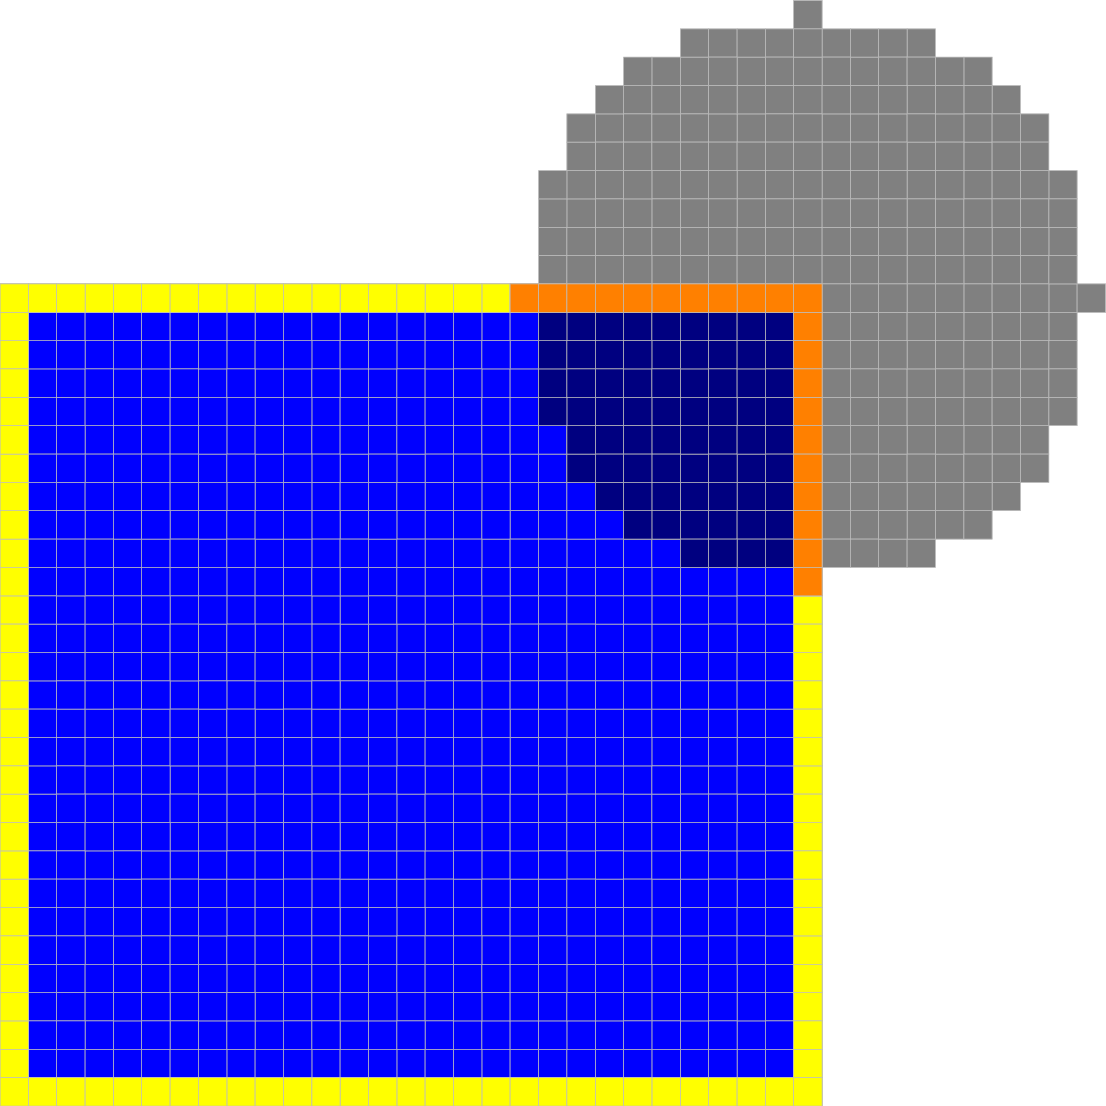
\includegraphics[scale=0.1]{figures/non-submodular-elastica/before-opt.png}\hspace{2em}
\only<1-2>{
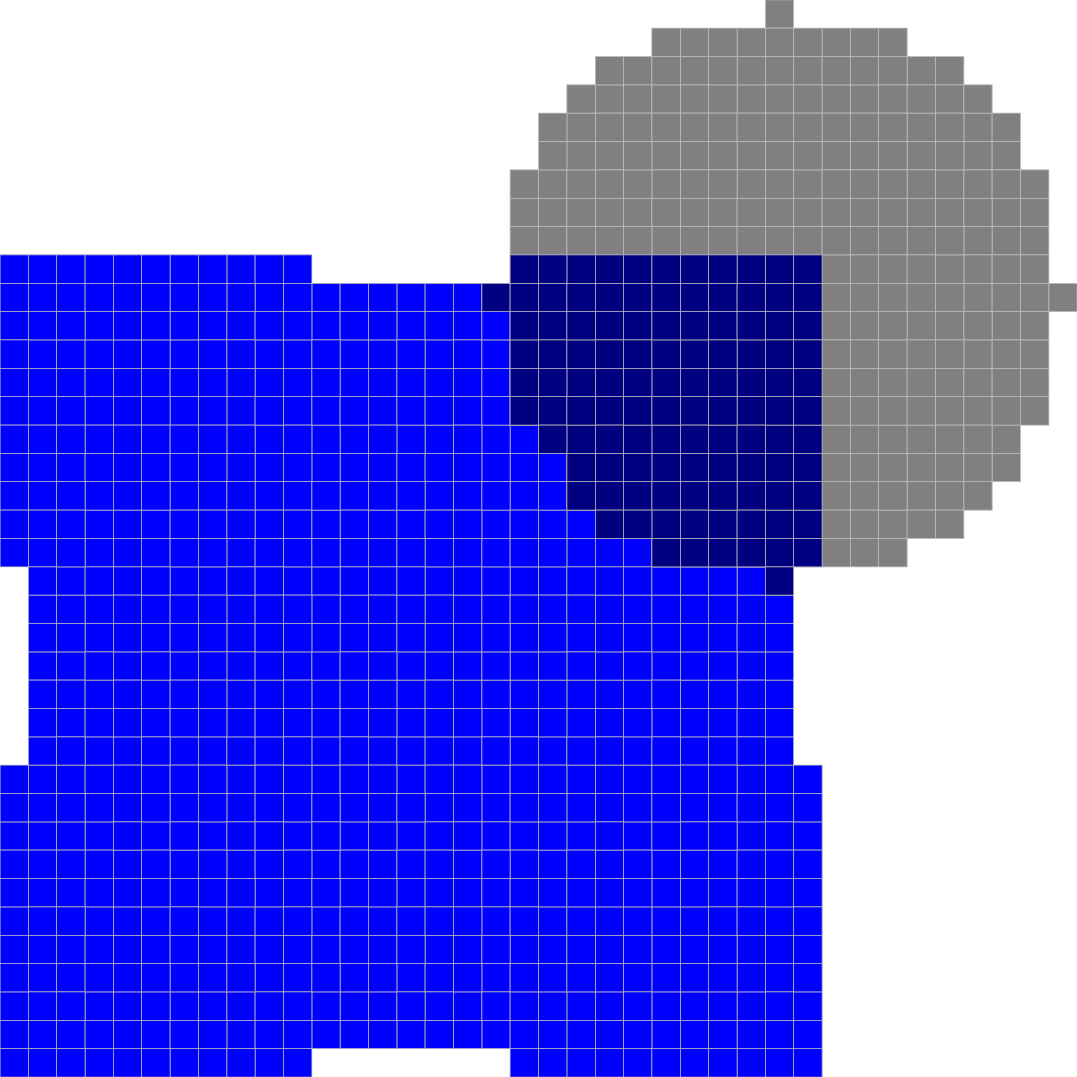
\includegraphics[scale=0.1]{figures/non-submodular-elastica/shape-opt-ball-after.png}}
\only<3>{
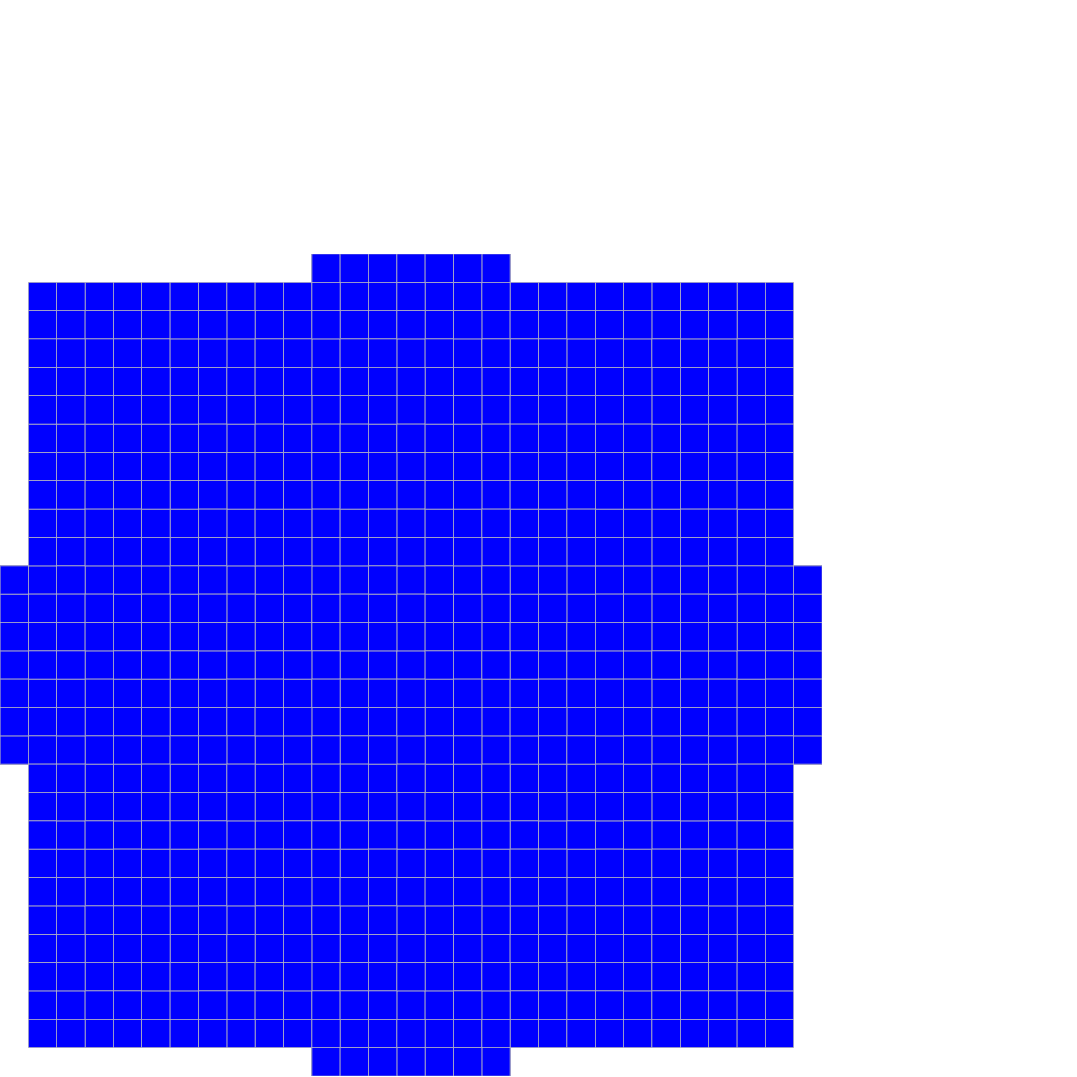
\includegraphics[scale=0.1]{figures/non-submodular-elastica/shape-opt-after-inverted.png}}
\end{minipage}

\begin{itemize}
\item{Optimization identifies zones of shortage (convex) or abundance (concave) of pixels.}
\onslide<2->{
\item{$x=1 \rightarrow$ Zone of shortage of pixels (convex) $\rightarrow$ Estimator disk should be shifted towards the interior $\rightarrow$ This pixel does not belong to the next contour. }}
\end{itemize}
\end{frame}

\begin{frame}
{Non-submodular elastica}
{FlipFlow}
\begin{minipage}[t][0.6\textheight][t]{1\textwidth}
\footnotesize
\only<1-6>{
\begin{align*}
  E_{(\vec{\theta},m)}^{flip}( \highlight{2}{1,3-5}{ \Ds^{(k)},X^{(k)} } ) =& \sum_{ x_j \in X^{(k)}}{ \alpha s(x_j)} +  \sum_{ p \in \highlight{3}{1-2,4-}{R_m(\Ds^{(k)})}}{\beta \hat{\kappa}(p)^2}\\ 
  \onslide<5->{=& \sum_{ x_j \in X^{(k)}}{ \alpha \highlight{6}{1-5,7-}{s(x_j)}} \\
  +&\sum_{ \substack{p \in \\ R_m(\Ds^{(k)})}}{ 2c_1 \beta  \Big( { (1/2+ |F_{r}^{(k)}(p)|-c_2) \cdot \sum_{ \substack{ x_j \in \\ X_{r}^{(k)}(p)}}{x_j} } + \sum_{ \substack{j<l, \\ x_j,x_l \in \\ X_{r}^{(k)}(p) } }{x_jx_l} \Big) }}
\end{align*}}
\only<7->{
\begin{align*}
  E_{(\vec{\theta},m)}^{flip}( \highlight{2}{1,3-5}{ \Ds^{(k)},{\highlight{7}{8-}{1-X^{(k)}} }} ) =& \sum_{ x_j \in X^{(k)}}{ \alpha s(x_j)} +  \sum_{ p \in \highlight{4}{1-3,5-}{R_m(\Ds^{(k)})}}{\beta \hat{\kappa}(p)^2}\\ 
  \onslide<5->{=& \sum_{ x_j \in X^{(k)}}{ \alpha \highlight{6}{1-5,7-}{s(x_j)}} \\
  +&\sum_{ \substack{p \in \\ R_m(\Ds^{(k)})}}{ 2c_1 \beta  \Big( { (1/2+ |F_{r}^{(k)}(p)|-c_2) \cdot \sum_{ \substack{ x_j \in \\ X_{r}^{(k)}(p)}}{x_j} } + \sum_{ \substack{j<l, \\ x_j,x_l \in \\ X_{r}^{(k)}(p) } }{x_jx_l} \Big) }}
\end{align*}}
\end{minipage}
%
%
\only<4>{
	\begin{figure}
	\begin{tikzpicture}[overlay, remember picture] 
	\node at (current page.center) 
	    [
	    anchor=center,
	    xshift=0mm,
	    yshift=0mm
	    ] 
	{
	
	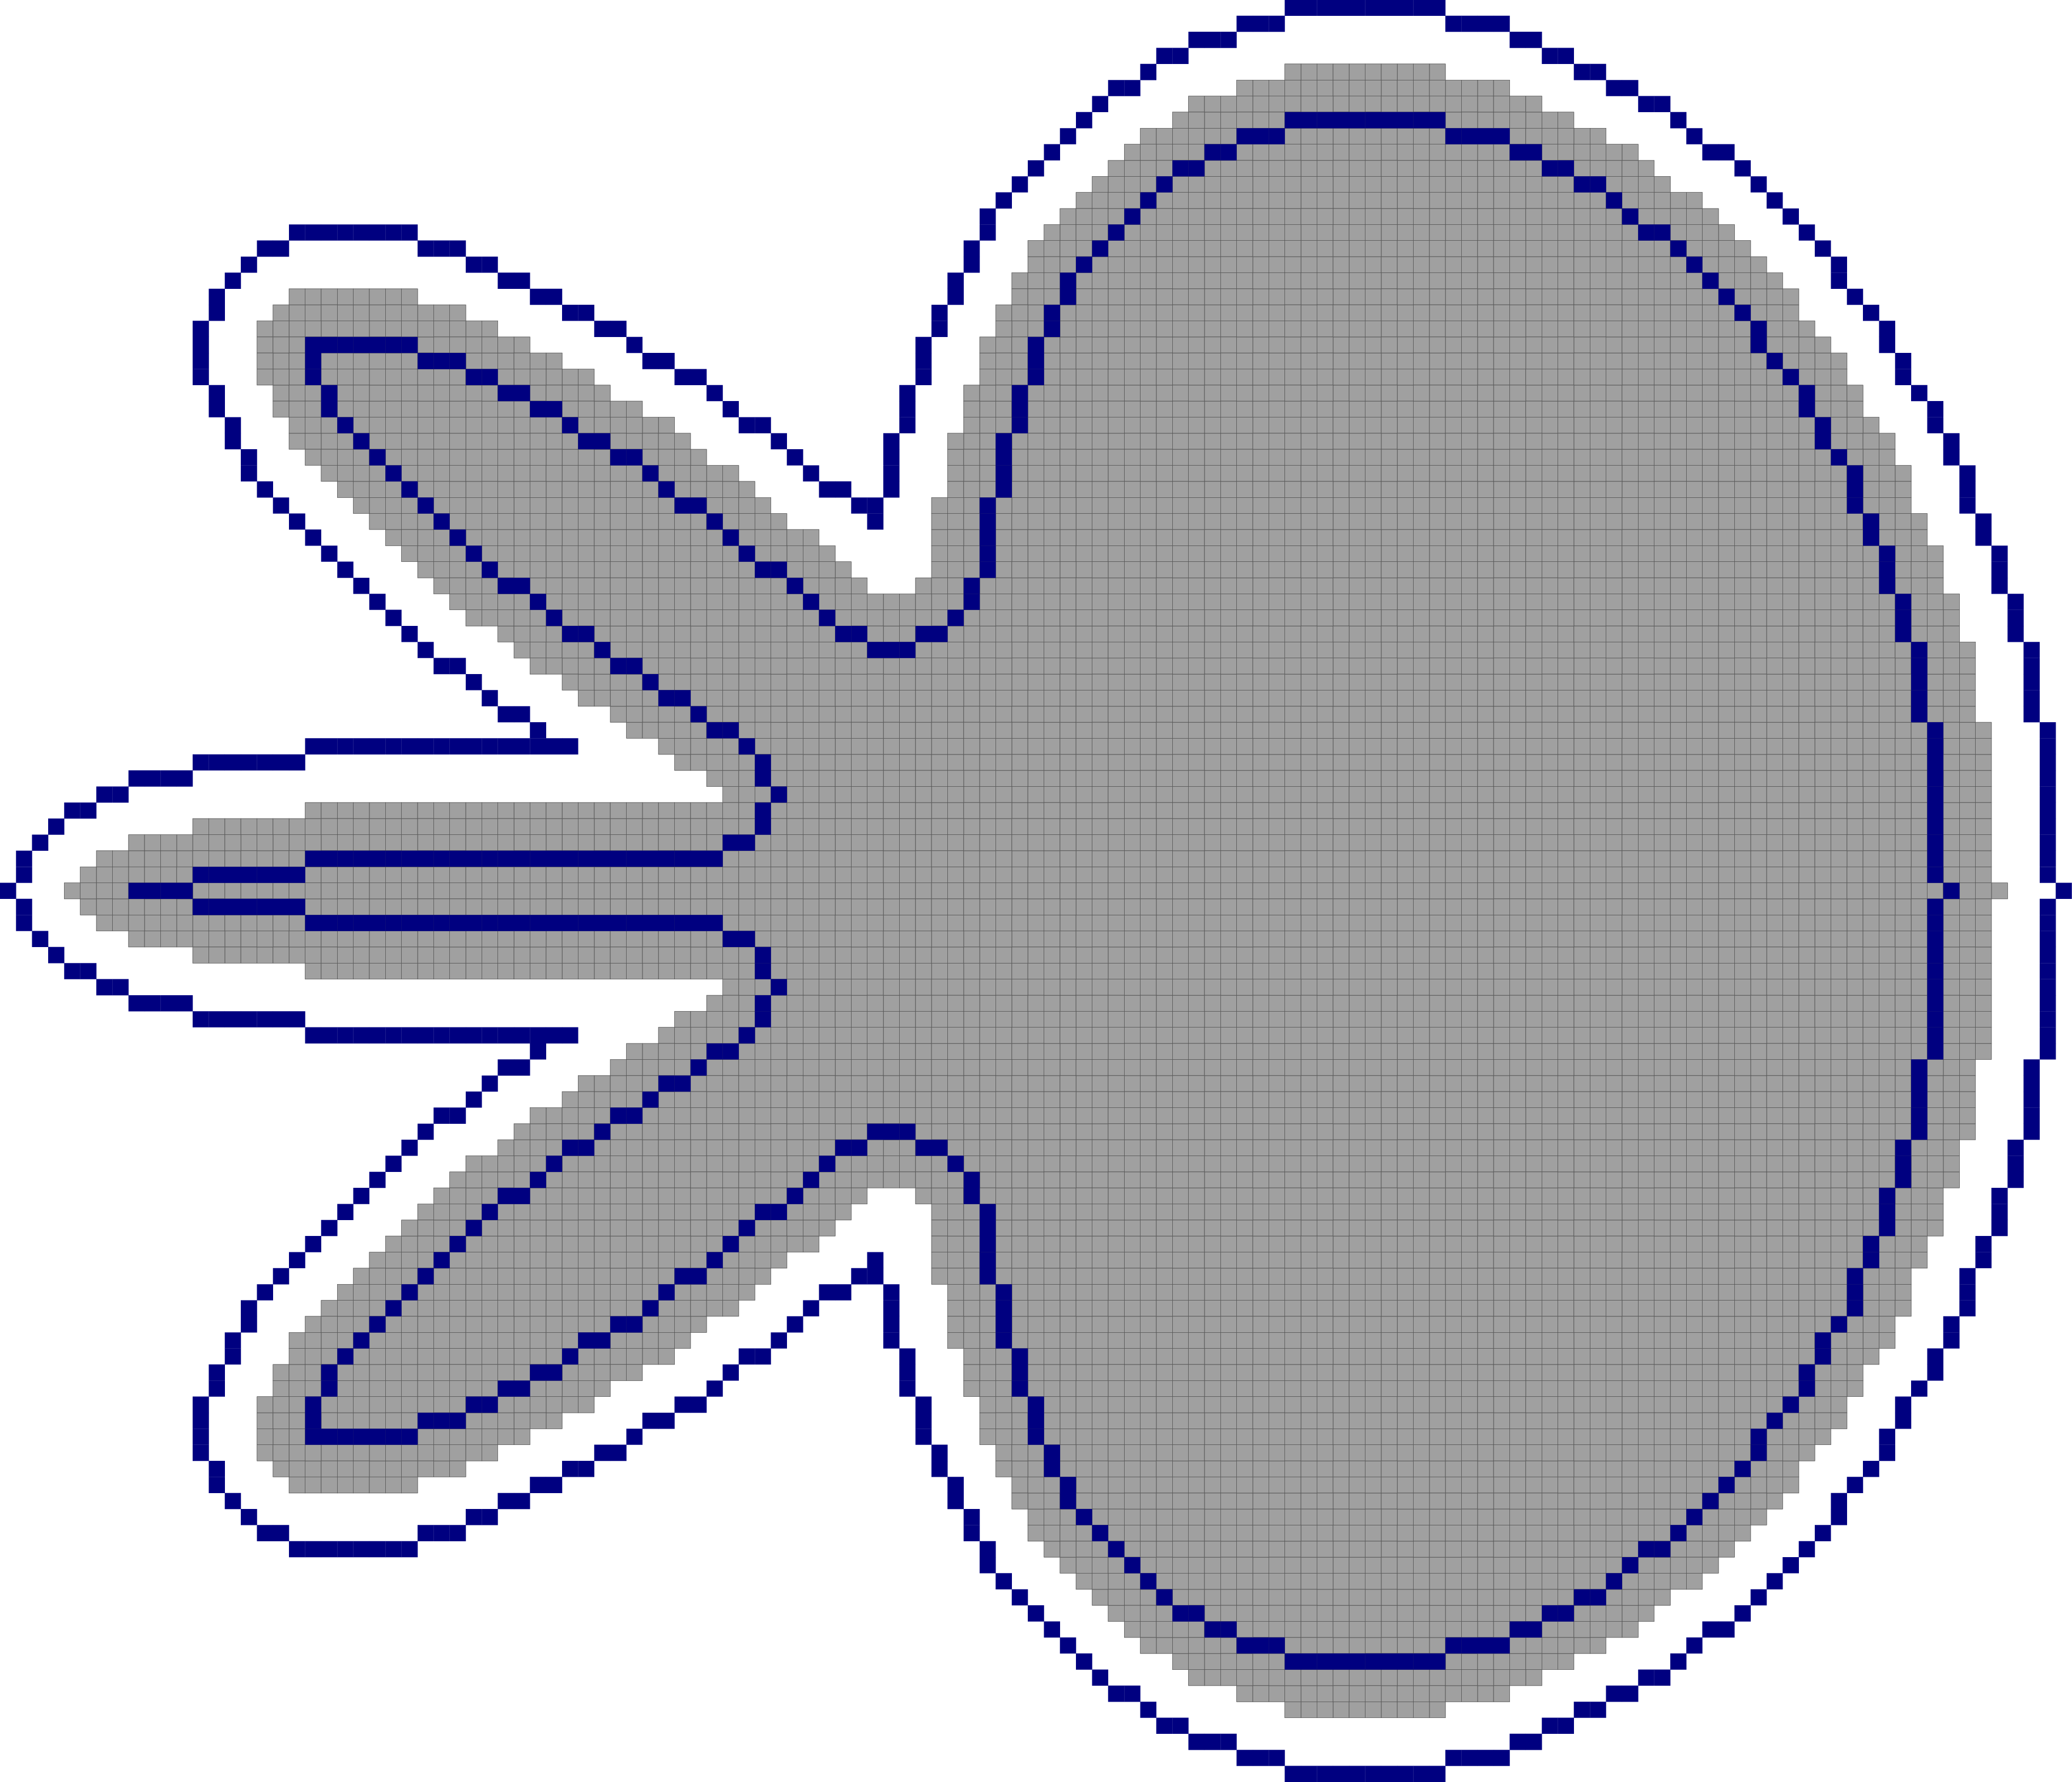
\includegraphics[scale=0.05]{figures/non-submodular-elastica/ring.png}
		
	};
	\end{tikzpicture}	
	\end{figure}}%
%
%
\begin{minipage}[t][0.39\textheight][t]{1\textwidth}
\only<2-4>{
\begin{center}
$\displaystyle
D \subset \Omega \subset \mathbb{Z}^2, \quad
X^{(k)} := \{ \; x_i \in \{0,1\} \; | \; p_i \in I^{(k)} \; \}$
\end{center}}
\only<3-4>{
\begin{center}
$\displaystyle
R_m(D) := \{ p \; | \; m-1 < d_D(p) \leq m \} \cup \{ p \; | \; -m+1 > d_D(p) \geq -m \}$
\end{center}}
\only<6>{
\begin{center}
\[
  s(x_j)=\sum_{q_i \in \mathcal{N}_4(p_j)}{ t(q_i) }, \quad \text{where } t(q_i) = \left\{\begin{array}{ll}
  (x_j-x_i)^2, & \text{if } q_i \in I^{(k)}\\
  (x_j-1)^2, & \text{if } q_i \in F^{(k)}\\
  (x_j-0)^2, & \text{otherwise. }
  \end{array}\right.
\]
\end{center}}
\only<7>{
\begin{center}
\[
  s(x_j)=\sum_{q_i \in \mathcal{N}_4(p_j)}{ t(q_i) }, \quad \text{where } t(q_i) = \left\{\begin{array}{ll}
  (x_j-x_i)^2, & \text{if } q_i \in I^{(k)}\\
  (x_j-{\color{blue}0})^2, & \text{if } q_i \in F^{(k)}\\
  (x_j-{\color{blue}1})^2, & \text{otherwise. }
  \end{array}\right.
\]
\end{center}}
\begin{minipage}{0.49\textwidth}
\scriptsize
\only<9->{\transparent{0.4}}
\only<8->{
\begin{center}
Shrink mode (convexities)
\[
\begin{array}{rl}
	a^{(k)} &\leftarrow \displaystyle \argmin_{X^{(k)}} E_{\vec{\Theta},m}^{flip}(D^{(k)},1-X^{(k)});\\[1.5em]
	D^{(k+1)} &\leftarrow F^{(k)} + a^{(k)}.
\end{array}
\]
\end{center}}
\end{minipage}
\begin{minipage}{0.49\textwidth}
\scriptsize
\only<9->{
\begin{center}
Expansion mode (concavities)
\[
\begin{array}{rl}
	a^{(k)} &\leftarrow 	\displaystyle \argmin_{\overline{X}^{(k)}} E_{\vec{\Theta},m}^{flip}(\overline{D}^{(k)},1-\overline{X}^{(k)});\\[1.5em]
	D^{(k+1)} &\leftarrow \overline{ \overline{F}^{(k)} + a^{(k)} }.
\end{array}
\]
\end{center}}
\end{minipage}
\end{minipage}

\end{frame}

\begin{frame}
{Non-submodular elastica}
{Evaluation on farther rings}

\begin{minipage}{0.49\textwidth}
\center
$r=3$\\
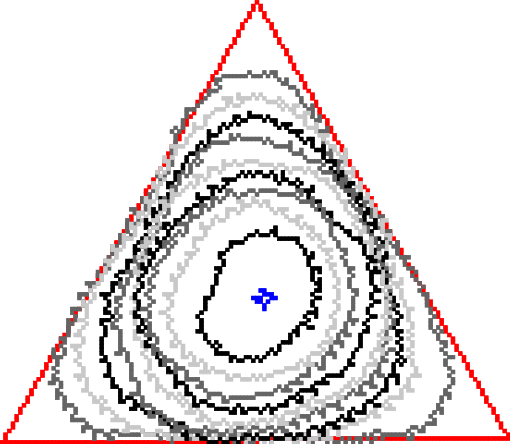
\includegraphics[scale=0.2]{figures/non-submodular-elastica/radius-effect/triangle-r3.png}\\[1em]
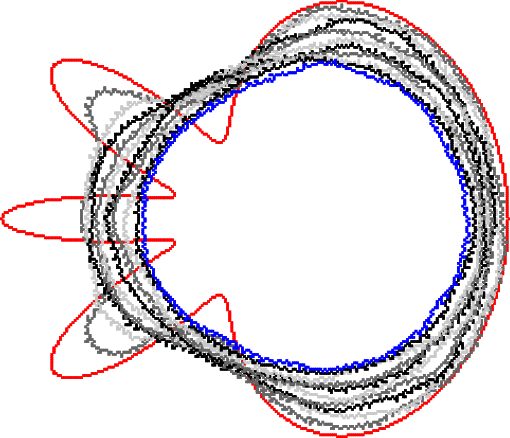
\includegraphics[scale=0.2]{figures/non-submodular-elastica/radius-effect/flower-r3.png}
\end{minipage}
\begin{minipage}{0.49\textwidth}
\center
$r=5$\\
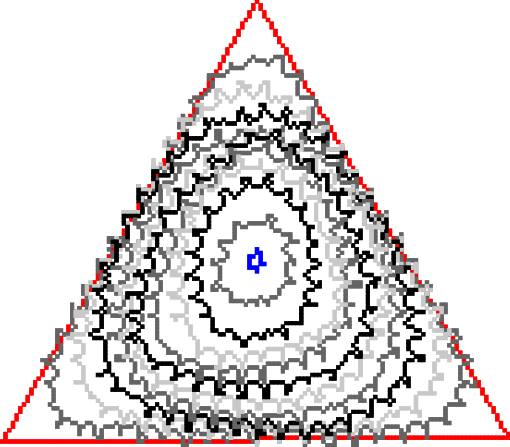
\includegraphics[scale=0.2]{figures/non-submodular-elastica/radius-effect/triangle-r5.png}\\[1em]
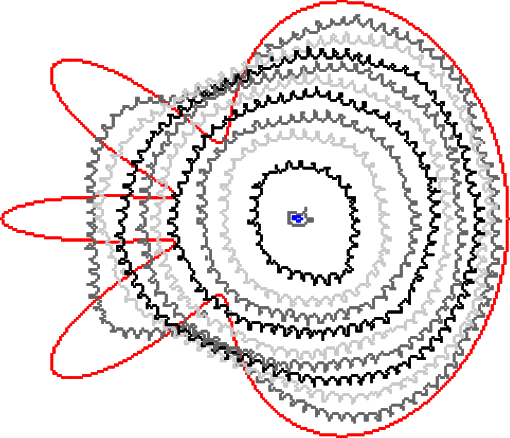
\includegraphics[scale=0.2]{figures/non-submodular-elastica/radius-effect/flower-r5.png}
\end{minipage}

\end{frame}

\begin{frame}
{Non-submodular elastica}
{Evaluation on farther rings}
\begin{tabular}{cccc}
\multicolumn{4}{c}{$r=5$}\\
$m=1$ & $m=3$ & $m=4$ & $m=5$ \\
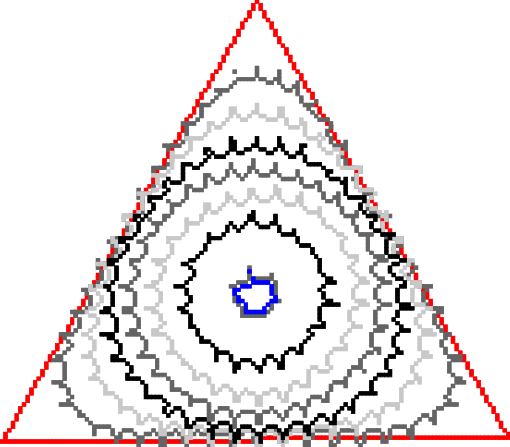
\includegraphics[scale=0.13]{figures/non-submodular-elastica/level-effect/triangle-l1.png}&
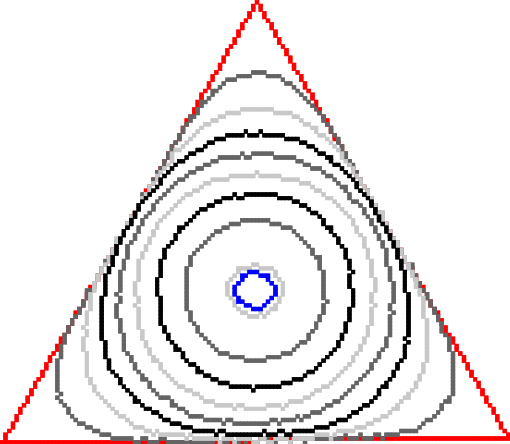
\includegraphics[scale=0.13]{figures/non-submodular-elastica/level-effect/triangle-l3.png}&
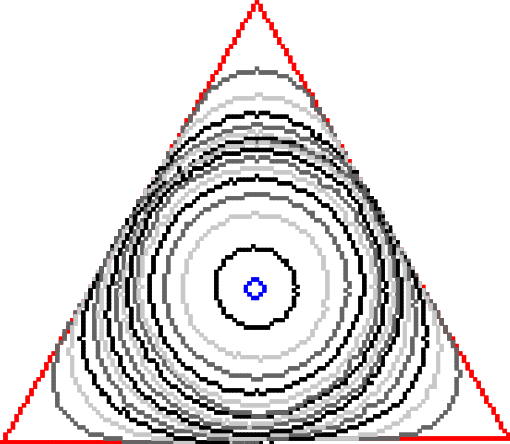
\includegraphics[scale=0.13]{figures/non-submodular-elastica/level-effect/triangle-l4.png}&
\includegraphics[scale=0.13]{figures/non-submodular-elastica/level-effect/triangle-l5.png}\\[2em]
\includegraphics[scale=0.13]{figures/non-submodular-elastica/level-effect/flower-l1.png}&
\includegraphics[scale=0.13]{figures/non-submodular-elastica/level-effect/flower-l3.png}&
\includegraphics[scale=0.13]{figures/non-submodular-elastica/level-effect/flower-l4.png}&
\includegraphics[scale=0.13]{figures/non-submodular-elastica/level-effect/flower-l5.png}
\end{tabular}
\end{frame}

\begin{frame}
{Non-submodular elastica}
{Contour correction}
\begin{tabular}{cc}
\includegraphics[scale=0.28]{figures/non-submodular-elastica/contour-correction/gc-seg-airplane.png}&
\includegraphics[scale=0.28]{figures/non-submodular-elastica/contour-correction/corrected-seg-airplane.png}\\[1em]
\includegraphics[scale=0.28]{figures/non-submodular-elastica/contour-correction/gc-seg-panther.png}&
\includegraphics[scale=0.28]{figures/non-submodular-elastica/contour-correction/corrected-seg-panther.png}
\end{tabular}
\end{frame}

\begin{frame}
{Non-submodular elastica}
{Unlabeled ratio}
\includegraphics[scale=0.28]{figures/non-submodular-elastica/level-effect/plot-unlabeled-triangle.png}\hspace{1em}
\includegraphics[scale=0.28]{figures/non-submodular-elastica/level-effect/plot-unlabeled-flower.png}

\begin{minipage}[t][0.5\textheight]{1\textwidth}
%
\only<2>{
\center
\begin{tabular}{cc}
$m=1$ & $m=3$\\[1em]
\includegraphics[scale=0.13]{figures/non-submodular-elastica/level-effect/triangle-l1.png}&
\includegraphics[scale=0.13]{figures/non-submodular-elastica/level-effect/triangle-l3.png}
\end{tabular}}%
%
\begin{itemize}
{\only<4->{\transparent{0.4}}
\onslide<3->{\item{Given that we evaluate the curvature estimator on the \emph{initial contour}, how pixels should change with respect this contour to reduce the difference of inner and outer pixels?}}
}
\onslide<4->{\item{Given that the shape does not change, where the estimation disks should be centered in order to reduce the difference of inner and outer pixels?}}
\end{itemize}%
%
\end{minipage}


\end{frame}

\begin{frame}
{Non-submodular elastica}
{Balance coefficient}
\begin{minipage}{0.5\textwidth}
\center
\includegraphics[scale=0.2]{figures/non-submodular-elastica/balance-coefficient-zero-level-set.png}
\end{minipage}
\begin{minipage}{0.49\textwidth}
\footnotesize
\begin{itemize}
\item{Balance coefficient}
\begin{align*}
u_r(D,p) &= \left( \frac{\pi r^2}{2} - |B_r(p) \cap D| \right)^2
\end{align*}
\item{White contour: contour of the shape}
\item{Pink contour: zero level set of the balance coefficient}
\end{itemize}
\end{minipage}
\end{frame}

\begin{frame}
{Non-submodular elastica}
{Conclusion}

\begin{itemize}
\item{Change pixels in current contour to reduce the difference between inner and outer pixels.}
\item{Quadratic non-submodular energy.}
\pause
\item{Farther rings: better results when disks are evaluated farther from the contour. }
\pause
\item{Pos-processing procedure: contour correction. }
\pause\vspace{1em}

\textbf{How to explain perturbations?}

\item{Unstable hypothesis: fixing the contour (dimension 1) is more sensitive than fixing the shape (dimension 2).}
\item{Make the shape evolve to the zero level set of its balance coefficient.}
\end{itemize}
\end{frame}


%\begin{align*}
%  s(x_{w(p)})=\sum_{q \in \mathcal{N}_4(p)}{ t(q) }, \quad \text{where } t(q) = \left\{\begin{array}{ll}
%  (x_{w(p)}-x_{w(q)})^2, & \text{if } q \in I^{(k)}\\
%  (x_{w(p)}-1)^2, & \text{if } q \in F^{(k)}\\
%  (x_{w(p)}-0)^2, & \text{otherwise. }
%  \end{array}\right.
%\end{align*}
\section{Elastica minimization via graph-cuts}

\begin{frame}
\huge
Elastica minimization via graph-cuts
\end{frame}

\begin{frame}
{Elastica minimization via graph-cuts}
{Graph cut}
\center
\only<1>{
\includegraphics[scale=0.25]{figures/graphcut/cut-1.png}}%
\only<2>{
\includegraphics[scale=0.25]{figures/graphcut/cut-2.png}}%
\only<3>{
\includegraphics[scale=0.25]{figures/graphcut/cut-3.png}}%
\end{frame}

\begin{frame}
{Elastica minimization via graph-cuts}
{Zero level set of balance coefficient}
\center
\includegraphics[scale=0.25]{figures/non-submodular-elastica/balance-coefficient-zero-level-set.png}
\end{frame}

\begin{frame}
{Elastica minimization via graph-cuts}
{Building the graph}

\begin{minipage}{0.3\textwidth}
\only<1>{
\includegraphics[scale=0.5]{figures/graphcut/graph-model-1.png}}%
\only<2-4>{
\includegraphics[scale=0.5]{figures/graphcut/graph-model-2.png}}%
\only<5->{
\includegraphics[scale=0.5]{figures/graphcut/graph-model-3.png}}%
\end{minipage}
%
%
\begin{minipage}{0.69\textwidth}
\footnotesize
\begin{itemize}
\onslide<2->{\item{Optimization band
\begin{align*}
\only<2>{O_n(D) :=& \{ p \in D \; | \; -n \leq d_D(p) \leq n \} \\}
\only<3->{O(D) :=& \{ p \in D \; | \; -n \leq d_D(p) \leq n \} \\}
\onslide<4->{F(D) :=& D \setminus O(D)}
\end{align*}}}
\onslide<5->{\item{Graph $\mathcal{G}_D(\mathcal{V},\mathcal{E},c)$
\begin{align*}
\mathcal{V} &= \{ v_p \; | \; p \in O(D) \} \cup \{s,t\} \\
\highlight{7}{5,6,8-}{\mathcal{E}} &= \highlight{7}{5,6,8-}{\{ \{v_p,v_q\} \; | \; p,q \in O(D) \text{ and } q \in \mathcal{N}_4(p) \}} \cup \highlight{6}{5,7-}{\mathcal{E}_{st}} \\
\highlight{6}{5,7-}{\mathcal{E}_{st}} &= \highlight{6}{5,7-}{\{ (s,v_p), (v_p,t) \; | \; p \in O(D) \}}
\end{align*}}}
\onslide<8->{\item{Edge's weight
\begin{center}
\begin{tabular}{|c|c|}
\hline
\textbf{edge} $e$ & $\mathbf{c(e)}$\\
\hline
$\{v_p, v_q\}$ & $ u_r(D,p) + u_r(D,q) $\\
\hline
$(s,v_p)$ & $M$\\
\hline
$(v_p, t)$ & $M$\\
\hline
\end{tabular}
\end{center}
}}
\onslide<9->{\item{Digital shape update
\begin{align*}
D^{(k+1)} &= F(D^{(k)}) + S^{(k)}
\end{align*}}}
\end{itemize}
\end{minipage}
\end{frame}
%
%
%
\begin{frame}
{Elastica minimization via graph-cuts}
{Shape evolution}
\center
\onslide<2->{Stop if elastica increases $(\alpha=1/22^2,\beta=1)$\\[1em]}
\only<1>{
\begin{tabular}{cc}
\includegraphics[scale=0.12]{figures/graphcut/no-neighborhood-flow/triangle-scaled.png}\hspace{3em} &
\includegraphics[scale=0.12]{figures/graphcut/no-neighborhood-flow/square-scaled.png}\\[2em]
\includegraphics[scale=0.12]{figures/graphcut/no-neighborhood-flow/flower.png}\hspace{3em} &
\includegraphics[scale=0.12]{figures/graphcut/no-neighborhood-flow/bean.png}
\end{tabular}}
\only<2>{
\begin{tabular}{cc}
\includegraphics[scale=0.12]{figures/graphcut/no-neighborhood-flow-always-improve/triangle.png}\hspace{3em} &
\includegraphics[scale=0.12]{figures/graphcut/no-neighborhood-flow-always-improve/square.png}\\[2em]
\includegraphics[scale=0.12]{figures/graphcut/no-neighborhood-flow-always-improve/flower.png}\hspace{3em} &
\includegraphics[scale=0.12]{figures/graphcut/no-neighborhood-flow-always-improve/bean.png}
\end{tabular}}
\end{frame}

\begin{frame}
{Elastica minimization via graph-cuts}
{The $a$-probe set}

\begin{definition}[$a$-probe set]
	Let $\Ds \subset \Omega \subset \mathbb{Z}^2$ a digital set and $a$ a natural number. The $a$-probe set of $\Ds$ is defined as
	\begin{align*}
		\mathcal{P}_a(\Ds) &= \Ds \cup \bigcup_{a' < a}{\Ds^{+a'} \cup \Ds^{-a'}},
	\end{align*}
	where $\Ds^{+a}$($\Ds^{-a}$) denotes a dilation(erosion) by a disk of radius $a$.
\end{definition}

\textbf{Candidate selection}
\[\begin{array}{l}
	sol(D^{(k)}) \longleftarrow \bigcup_{D' \in \mathcal{P}_a(D^{(k)})} \Big\{ F^{(k)} + S  \; | \; mincut(S,\mathcal{G}_{D'}) \Big\} 	
\end{array}
\]

\textbf{Candidate validation}
\[\begin{array}{l}
\Ds^{(k+1)} \longleftarrow \displaystyle \argmin_{ D' \in sol(D^{(k)}) }{ \hat{E}_{\vec{\theta}}(D')}
\end{array}
\]

\end{frame}

\begin{frame}
{Elastica minimization via graph-cuts}
{Shape evolution with $a$-probe set}

\center
\only<1>{Stop if elastica increases $(\alpha=1/22^2,\beta=1)$ \\[1em]}
\only<2>{Always update $(\alpha=1/22^2,\beta=1)$ \\[1em]}
\only<1>{
\begin{tabular}{cc}
\includegraphics[scale=0.12]{figures/graphcut/with-neighborhood-flow-always-improve/triangle.png}\hspace{3em} &
\includegraphics[scale=0.12]{figures/graphcut/with-neighborhood-flow-always-improve/square.png}\\[2em]
\includegraphics[scale=0.12]{figures/graphcut/with-neighborhood-flow-always-improve/flower.png}\hspace{3em} &
\includegraphics[scale=0.12]{figures/graphcut/with-neighborhood-flow-always-improve/bean.png}
\end{tabular}}
%
%
\only<2>{
\begin{tabular}{cc}
\includegraphics[scale=0.12]{figures/graphcut/with-neighborhood-flow/radius_16/triangle.png}\hspace{3em} &
\includegraphics[scale=0.12]{figures/graphcut/with-neighborhood-flow/radius_16/square.png}\\[2em]
\includegraphics[scale=0.12]{figures/graphcut/with-neighborhood-flow/radius_16/flower.png}\hspace{3em} &
\includegraphics[scale=0.12]{figures/graphcut/with-neighborhood-flow/radius_16/bean.png}
\end{tabular}}
\end{frame}

\begin{frame}
{Elastica minimization via graph-cuts}
{Shape evolution with $a$-probe set}

\begin{minipage}{0.25\textwidth}
\center
\includegraphics[scale=0.06]{figures/graphcut/with-neighborhood-flow/radius_16/triangle.png}\\[1em]
\includegraphics[scale=0.06]{figures/graphcut/with-neighborhood-flow/radius_16/square.png}\\[1em]
\includegraphics[scale=0.06]{figures/graphcut/with-neighborhood-flow/radius_16/flower.png}\\[1em]
\includegraphics[scale=0.06]{figures/graphcut/with-neighborhood-flow/radius_16/bean.png}
\end{minipage}%
%
%
\begin{minipage}{0.74\textwidth}
\center
\includegraphics[scale=0.18]{figures/graphcut/with-neighborhood-flow/plots/elastica.png}\\
\includegraphics[scale=0.18]{figures/graphcut/with-neighborhood-flow/plots/bars.png}
\end{minipage}
\end{frame}

\begin{frame}
{Elastica minimization via graph-cuts}
{Contour correction}

\begin{minipage}{0.5\textwidth}
\center
\only<1>{
\includegraphics[scale=0.45]{figures/graphcut/contour-correction/cat/gc-seg.png}

Initial segmentation

}%
\only<2>{
\includegraphics[scale=0.45]{figures/graphcut/contour-correction/vase/gc-seg.png}

Initial segmentation

}%
\only<3,4>{
\includegraphics[scale=0.4]{figures/graphcut/contour-correction/coala/gc-seg.png}

Initial segmentation

}%
\end{minipage}%
\begin{minipage}{0.5\textwidth}
\center
\only<1>{
\includegraphics[scale=0.45]{figures/graphcut/contour-correction/cat/corrected-seg.png}

$0.825s$ ($3$ it)

}%
\only<2>{\includegraphics[scale=0.45]{figures/graphcut/contour-correction/vase/corrected-seg.png}

$0.746s$ ($3$ it)

}%
\only<3>{\includegraphics[scale=0.4]{figures/graphcut/contour-correction/coala/5it.png}

$1.1s$ ($3$ it)

}%
\only<4>{\includegraphics[scale=0.4]{figures/graphcut/contour-correction/coala/30it.png}

$10s$ ($30$ it)

}%
\end{minipage}%

\end{frame}

\begin{frame}
{Elastica minimization via graph-cuts}
{Contour completion}

\begin{minipage}[t][0.47\textheight]{1\textwidth}
\center
\includegraphics[scale=0.28]{figures/graphcut/contour-completion/green-snake/gc-seg.png}

Initial segmentation

\end{minipage}
\vspace{1em}
\begin{minipage}[t][0.47\textheight]{1\textwidth}
\center
\includegraphics[scale=0.28]{figures/graphcut/contour-completion/green-snake/corrected-seg.png}

$17s$ ($62$ it)

\end{minipage}


\end{frame}


\begin{frame}[allowframebreaks]
    \frametitle{References}	
    \printbibliography
\end{frame}


\end{document}